\let\textcircled=\pgftextcircled
\chapter{Markov state model optimization}\label{chap:msm}

\section{Introduction}


% \caption{Atomic structure of Alanine dipeptide (AD). The cylinders represent chemical bonds and their intersections represent atoms. Grey, blue, red and white colors are carbon, nitrogen, oxygen and hydrogen atoms respectively. The atoms involved in the $\phi, \psi$ dihedral angles are labeled and highlighted as spheres.  The $\phi$ angle is formed from the intersection of the planes formed by the atoms (C\textsubscript{1}, N, CA) and (N, CA, C\textsubscript{2}).  The $\psi$ angle is formed from the planes formed by the atoms (N, CA, C\textsubscript{2}) and (CA, C\textsubscript{2}, O).}\label{fig:ala2}

\begin{table}
    \centering
    \caption[Important symbols]{\textsc{Important symbols used throughout this chapter}.}
    \begin{tabularx}{0.9\textwidth}{ l >{\raggedright\arraybackslash}X  } 
    \hline
        \textbf{Symbol}  &  \textbf{Definition} \\
        \hline\hline
        $\mathbf{x}$ & vector of MSM hyperparameters \\
        $\chi$ & MSM hyperparameter: a protein/peptide feature e.g., backbone torsion \\
        $\tau$ & MSM hyperparameter: the TICA lag time \\
        $m$ & MSM hyperparameter: the number of TICA components retained \\
        $n$ & MSM hyperparameter: the number cluster centers. \\
        $y$ & the response of an MSM, $y =\operatorname{VAMP-2}$ \\
        $\Psi_i(\mathbf{z})$ & the right eigenfunction of an MSM \\
        $\delta_i$ & the discretisation error of the MSM eigenfunction $\Psi_{i}$ \\
        % $g(\mathbf{x})$ & the objective function. In the case of MSMs this is the unknown function 
        %                     which maps hyperparameters to the response. \\
        $f(\mathbf{x})$ & response surface function, a statistical estimation the objective function 
                          which is easy to optimise. In the context of Bayesia optimisation called the 
                          surrogate function. \\
        $\mathcal{D}_{N}$ & a hyperparameter trial data set. A set of $N$ hyperparameter/response pairs: $(\mathbf{x}_{i}, y_{i})$. Used to estimate the response surface. \\
        $\tau_{\mathrm{M}}$ & the MSM lag time.  \\
        $\mu(\mathbf{x})$ & the mean function of a Gaussian Process. \\
        $k(\mathbf{x}, \mathbf{x}^{\prime})$ & the covariance kernel of a Gaussian Process. Defines the covariance between the response at $\mathbf{x}$ and $\mathbf{x}^{\prime}$. \\
        $\mathbf{K}$ & the covariance matrix of the Gaussian Process. $K_{ij} =k(\mathbf{x}_{i}, \mathbf{x}_{j})$. \\
        $\theta$ & the collection of kernel hyperparameters. \\
        $\eta$ & Kernel hyperparameter: determines the scale of fluctuations of the response. \\
        $\sigma_{n}$ & Kernel hyperparameter: determines the noise associated with a single trial. \\
        $l_{i}$ & Kernel hyperparameter: the characteristic length-scale of the Gaussian process 
                along the $i$th predictor (MSM hyper-hyperparameter).\\
        $R_{i}$ & Kernel hyperparameter: the relevance of the $i$th predictor, $R=\frac{1}{l}$. \\ 
        $\sigma(\mathbf{x})$ & the width of the Gaussian process at the point $\mathbf{x}$. These values  are the diagonal elements of $\mathbf{K}$. Depending on context this may or may not include the contribution from $\sigma_{n}$. \\
        $\alpha_{EI}(\mathbf{x})$ & the expected improvement acquisition function used to determine the next hyperparameter trial. \\
        $(\phi, \psi)$ & peptide feature: the backbone torsional angles of an amino acid.  \\
        $(\phi, \psi, \chi)$ & peptide feature: the backbone and residue torsional angles of an amino acid. \\
        $|\mathbf{r}_{1}-\mathbf{r}_{2}|$ & peptide feature: all heavy atom interatomic distances.  \\
        $(x, y, z)$ & peptide feature: Cartesian coordinates \\
        $C_{\alpha}-C_{\alpha}$ & peptide feature: the alpha carbon contact distances \\
        $X-X$ & peptide feature: the heavy atom contact distances \\
     \hline
     \end{tabularx}
    \label{tab:msm_symbols}
\end{table}

In chapter \ref{chap:theory} the theory of modelling biomolecular dynamics as a Markov process using a Markov state models (MSMs) was laid out. Central to the method is defining  a series of basis sets, $s^i,\ i=1, ..., n$, which  map atomic coordinates to $n$ discrete microstates. These basis sets allow the molecular dynamics trajectories to be represented as an approximate one-dimensional Markov chain from which the MSM can be estimated. The choice of basis set are crucial for accurately capturing the dynamics of system and must therefore be chosen with care \cite{husicOptimizedParameterSelection2016}. In section \ref{sec:theory_msm} the process of creating basis sets was described as using four (although many more are possible) modelling choices, or  \emph{hyperparameters}, collectively denoted by $\mathbf{x} = (\chi, \tau, m, n)$. Even within reasonable ranges of these hyperparameters, trying each distinct value of $\mathbf{x}$ is computationally intractable. A systematic method is needed to choose appropriate hyperparameters which is reproducible, makes maximum use of the available information, and with the least amount of computational effort. This chapter addresses this need by applying ideas and techniques from the machine learning literature, Bayesian optimisation and response surface methods, and applying them to the test system alanine dipeptide. 

Choosing hyperparameters can be thought of as an optimisation problem \cite{feurer2019hyperparameter,jonesEfficientGlobalOptimization1998}, where the task is to find  vectors from hyperparameter configuration space, $X=\chi \times \tau \times m \times n$  which maximise an objective function, $f$:  
\begin{equation}
    f: X \rightarrow \operatorname{VAMP-2}
\end{equation}
Within the MM community, efficiently finding the optimum set has recently gained attention \cite{schererVariationalSelectionFeatures2019}, however nine out of ten recent studies from a non-random sample\footnote{10 papers published in 2020 which cite PyEMMA \cite{schererPyEMMASoftwarePackage2015a} and apply MMs to understand a simulated data set.} performed no hyperparameter optimisation at all.  

Within the larger machine learning community, however, finding the optimum set of hyperparameters for a given model and data set is a common task and has received a lot of attention, as discussed in section \ref{sec:intro_hyper_opt} of the introduction. Much of the focus has been on creating algorithms which automatically optimise hyperparameters rather than a domain expert choosing the values ``by hand'' \cite{feurer2019hyperparameter}.  Automated methods of selecting hyperparameters are beneficial for a number of reasons as they \cite{feurer2019hyperparameter}:
\begin{enumerate}
    \item reduce the human and energy resources needed for creating an accurate model,
    \item improve the performance of model in general,
    \item improve reproducibility and transparency in the model estimation process. 
\end{enumerate}
There are two general approaches to hyperparameter optimisation: i) model-free and ii) model-based optimisation \cite{feurer2019hyperparameter}. 

\emph{Model-free} optimisation techniques include \cite{feurer2019hyperparameter}: grid search (or full-factorial design \cite{c1997montgomery}, i.e., placing a regular grid over the hyperparameter search space and evaluating each point), random search (i.e., randomly sampling hyperparameters from the search space)  and population techniques. The latter include evolutionary algorithms \cite{simon2013evolutionary},  particle swarm optimisation \cite{kennedyParticleSwarmOptimization1995,eberhart1998comparison} and covariance matrix adaption \cite{hansenCMAEvolutionStrategy2016}.  When hyperparameter optimisation is performed within the MM community, the former two methods are popular. For example, in reference \cite{husicOptimizedParameterSelection2016} the authors use random search to determine trends and heuristics for creating MSMs of fast folding proteins, while the authors of reference \cite{chenDynamicConformationalLandscape2019} used grid search over different protein features, various TICA hyperparameters, and number of microstates to optimise a MSM to describe the conformational landscape of the methyltransferase, SETD8. Random search has a number of advantages over grid search. First, when only a small proportion of the hyperparameters are relevant for determining the model score, random search has been shown  to be more efficient than  than grid search \cite{bergstrajamesbergstraRandomSearchHyperParameter2012}. The reason is that grid search places equal importance on each hyperparameter and effectively wastes the computational budget on combinations of hyperparameters which will score similarly. Second, it is easily adapted to parallel computer architectures and third, increasing the optimisation `budget' (the number of optimisation steps available) or the size of the search space is easily incorporated into the workflow \cite{feurer2019hyperparameter}.

\begin{figure}
    \centering
    \caption[Response surface and acquisition functions]{\textsc{Response surface and acquisition functions}. Panel (a) shows the elements of the hyperparameter trial data set, $\mathcal{D}$, as black crosses, the objective function $f(x)$ (black dashed line), and the estimated response surface $\hat{f}(x)$ (solid blue line) with uncertainty (shaded blue area). The dotted line shows the incumbent, $\max{\left(f(x)\right)}\ x\in \mathcal{D}$. Panel (b) shows a two acquisition functions: the probability of improvement $\mathbb{P}(I>0)$ (orange line) and the expected improvement $\mathbb{E}[I]$ (green line). For reference the improvement function, $I(x)$ (blue line) is also shown. The maximum of the acquisition functions are denoted with a star. }
    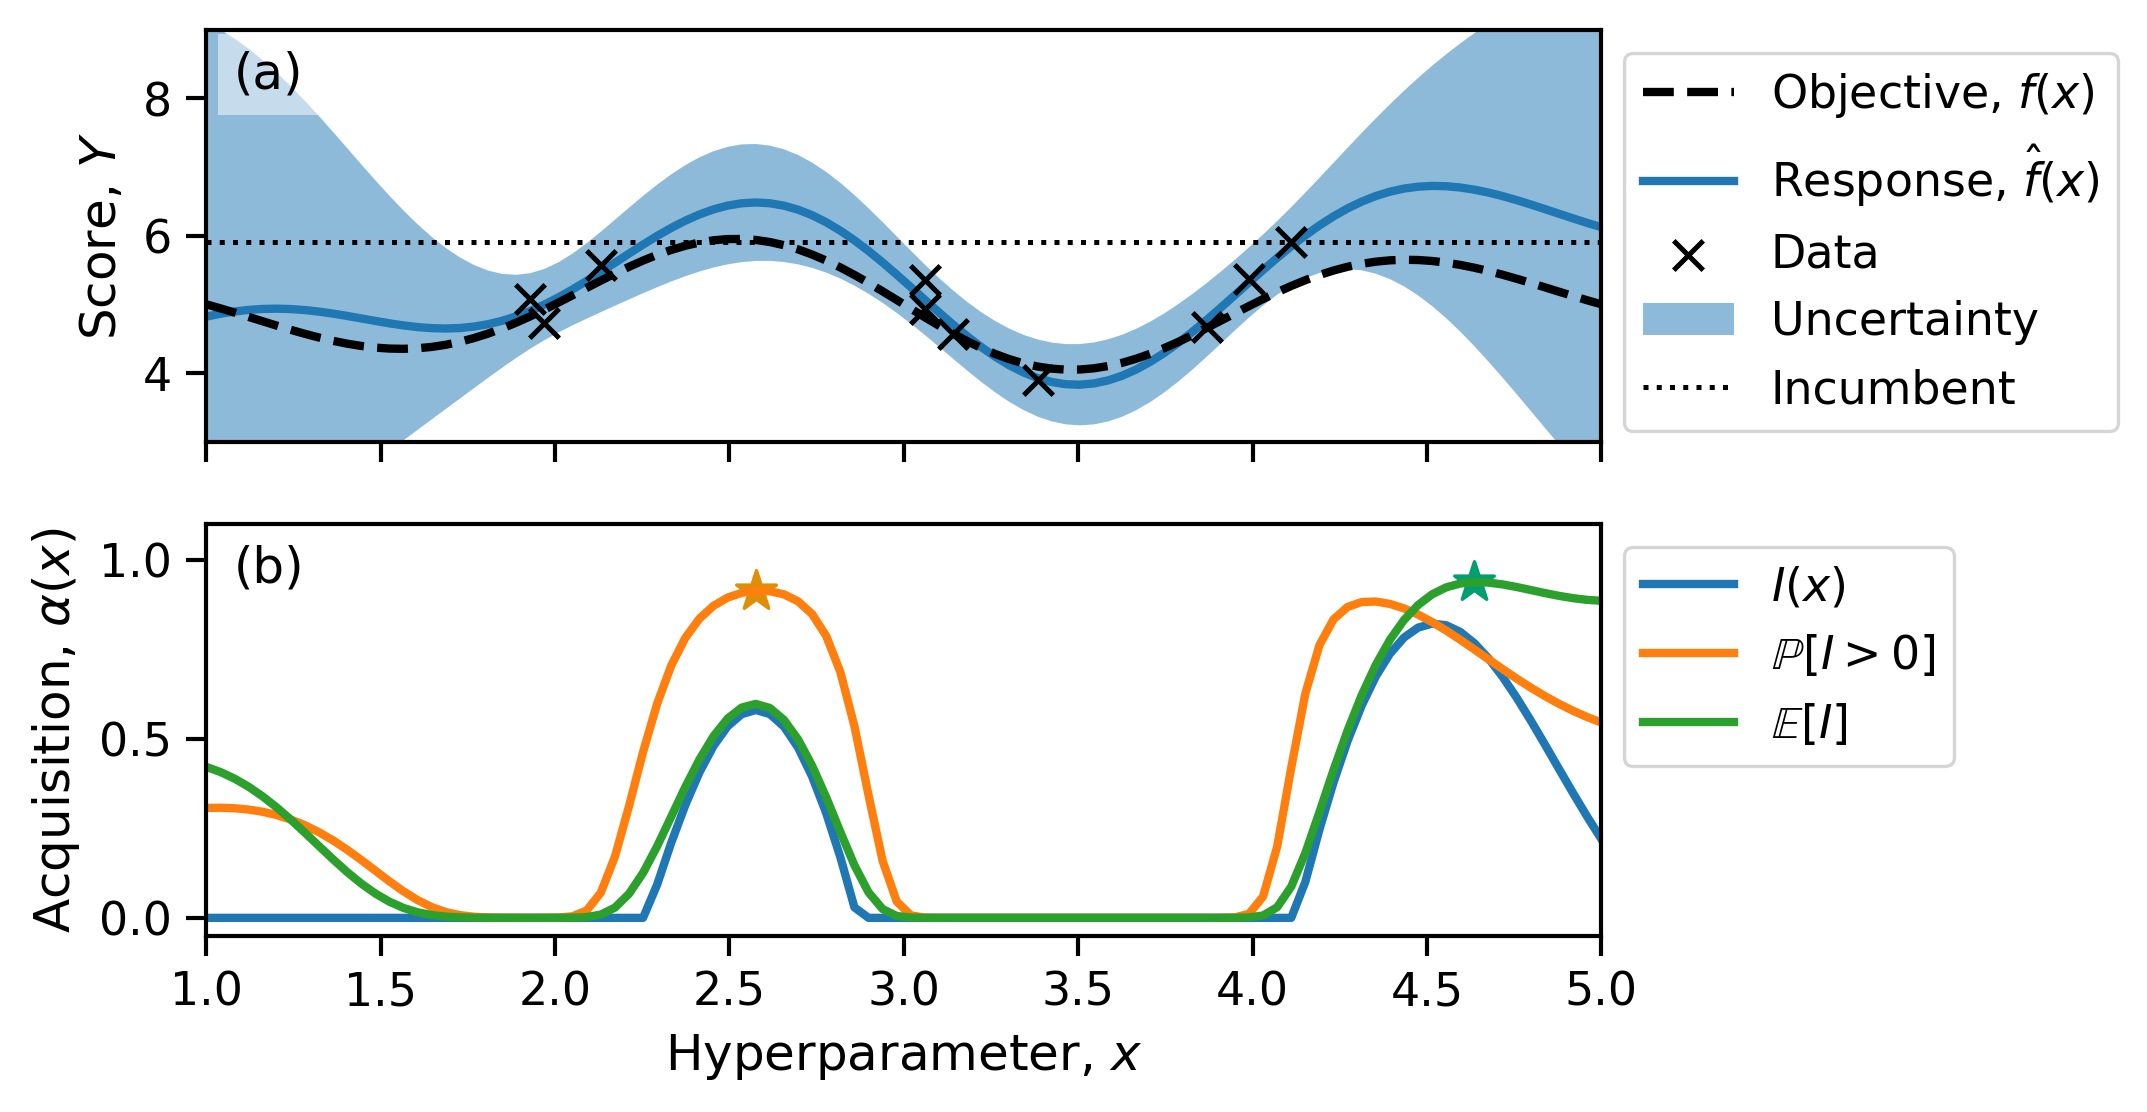
\includegraphics[width=0.8\textwidth]{chapters/msm_optimization/figures/response_surface_explainer.png}
    \label{fig:msm_rsm_explainer}
\end{figure}

\emph{Model-based} search techniques involve estimating a statistical approximation to the objective function, known  as the \emph{response surface} (or surrogate function) and using the response function to choose the next hyperparameter to evaluate \cite{hutterSequentialModelbasedOptimization2011}. The evaluated hyperparameter is then used to augment the data used to estimate the response surface \cite{hutterSequentialModelbasedOptimization2011}. The alternating sequence of response surface estimation and hyperparameter evaluation is continued until a satisfactory convergence in the maximum of the response surface is reached \cite{hutterSequentialModelbasedOptimization2011}. An example response surface for a model with a single hyperparameter is shown in figure \ref{fig:msm_rsm_explainer}. Evaluating the fictitious model with a hyperparameter value of $x$ leads to a model score of $y$. The pair $(x, y)$ will be referred to as a \emph{hyperparameter trial}. Repeating trials with different values of $x$ gives a (hyperparameter) \emph{trial data set}  $\mathcal{D}=\{(\mathbf{x}_{i}, y_{i})\}$. In the figure the elements of $\mathcal{D}$ are shown as black crosses. The score is a random variable, $Y$, which can be modelled by: $Y \sim f(x) + \epsilon$ where $\epsilon$ is an error term. The estimated function, $\hat{f}(x)$, is the response function and is shown as a blue line, while the uncertainty (as captured by $\epsilon$) is shown as a blue shaded area. The uncertainty arises from any random element in evaluating the score (e.g., from cross-validation) or from the model itself.  

Bayesian optimisation is a popular model-based technique for optimising hyperparameters \cite{bergstraAlgorithmsHyperParameterOptimizationa,hutterSequentialModelbasedOptimization2011,NIPS2012_4522,bergstraMakingScienceModel2013,feurer2019hyperparameter}. The key components of Bayesian optimisation are: i) the \emph{acquisition function}, $\alpha$, which determines the utility of choosing a particular hyperparameter value, and ii) the response function, which encapsulates all current knowledge of the objective function.  The next \emph{candidate} hyperparameter in the optimisation sequence is chosen by maximizing the acquisition function \cite{shahriariTakingHumanOut2016}. Acquisition functions trade-off exploration of the search space with exploitation of areas more likely to optimise the objective function. Each does this in their own way, with their own particular strengths and weaknesses, but they come in three main categories i) improvement-based policies, ii) optimistic policies, and iii) information-based policies \cite{shahriariTakingHumanOut2016}.

Improvement based policies use the improvement function, $I(\mathbf{x})$, (shown in figure \ref{fig:msm_rsm_explainer} panel (b) as the blue line), which is defined as the  difference between the value of the response surface, $f(\mathbf{x})$, and incumbent, $\mu^{*}$ \cite{shahriariTakingHumanOut2016}:
\begin{equation}
    I(\mathbf{x}):=\left(f(\mathbf{x}) - \mu^{*}\right) \mathbb{I}_{f(\mathbf{x}) > \mu^{*}}. 
\end{equation}
The incumbent \cite{brochuTutorialBayesianOptimization2010} is defined as $\mu^{*}=\max{\left(f(\mathbf{x})\right)},\ \mathrm{s.t.}\ \mathbf{x} \in \mathcal{D}$, and $\mathbb{I}$ is an indicator function which ensures that $I \ge 0$. In other words, the incumbent is optimum of the response surface but restricted to values of $\mathbf{x}$ which occur in the data used to estimate the response surface. Examples of such policies include probability of improvement \cite{Kushner1963} $\alpha_{\mathrm{PI}}(\mathbf{x}) = \mathbb{P}\left[I(\mathbf{x})>0\right]$  (orange line figure \ref{fig:msm_rsm_explainer} panel (b)) and the expected improvement \cite{mockus1978application} $\alpha_{\mathrm{EI}}(\mathbf{x}) = \mathbb{E}\left[I(\mathbf{x})\right]$ (green line in figure \ref{fig:msm_rsm_explainer} panel (b)). The probability of improvement tends to exploit known regions of the response surface and so can fail to explore sufficiently to find the global optimum \cite{jones2001taxonomy}. This is because, as can be seen from the definition, it treats all improvements the same no matter how small (although the incumbent can be altered to modify the explore/exploit trade-off) \cite{jones2001taxonomy}.  The expected improvement corrects this by taking into account both the probability of improvement \emph{and} the size of improvement. The difference between the two acquisition functions is demonstrated in figure \ref{fig:msm_rsm_explainer}. The improvement (blue line, panel (b)) has two peaks, a smaller peak at $x\simeq 2.6$ and a larger peak at $x\simeq 4.6$. The response function at $x\simeq 2.6$ has smaller uncertainty because of the larger number of observations surrounding it. The probability of improvement (orange line, panel (b)) measures the amount of uncertainty above the incumbent line (dotted line, panel (a)) and is greatest here as the majority of the blue shaded area is above the incumbent line. At $x\simeq 4.6$ and beyond, the uncertainty is large but more evenly distributed above and below the incumbent line, hence the probability of improvement peaks and then decreases. However, the expected improvement (green line) is large because the uncertainty in the response extends to high values of $y$ and the expectation is taken from above the incumbent line.  The expected improvement is a popular choice \cite{feurer2019hyperparameter} and is the default option in some well-known packages such as Spearmint \cite{NIPS2012_4522} and BayesOpt \cite{martinez-cantinBayesOptBayesianOptimization2014}. 

Optimistic policies, such as the upper confidence bound \cite{icml2010_129}, choose the candidate to maximize a particular quantile of the uncertainty in the response surface. They have been shown to minimize the `regret' accumulated over all iterations of the optimisation procedure \cite{icml2010_129}. The `regret' being the difference between the true maximum of the objective function and the objective function measured on the candidate hyperparameter trial \cite{berger2013statistical}. More detail on the performance of improvement and optimistic acquisition functions can be found in reference \cite{jones2001taxonomy}. Information based policies are based on the distribution over the potential hyperparameters, $p(\mathbf{x}|\mathcal{D})$, which describe the probability of optimising the objective function and are induced by the uncertainty in the response surface \cite{shahriariTakingHumanOut2016}. Examples include entropy search \cite{hennig2012entropy}, predictive entropy search \cite{hernandez2014predictive}, and entropy search portfolio \cite{shahriariEntropySearchPortfolio2015}.  


The second component of Bayesian optimisation is the functional form of the response function. Stochastic processes such as Gaussian processes (GPs) or T-student processes (TPs) \cite{rasmussenGaussianProcessesMachine2006} are common and are implemented in a number of packages \cite{martinez-cantinBayesOptBayesianOptimization2014,NIPS2012_4522,gpyopt2016,JMLR:v21:18-223,mcgibbonOspreyHyperparameterOptimization2016,liuAuptimizerExtensibleOpenSource2019}. Gaussian processes in particular have many useful properties for Bayesian optimisation \cite{feurer2019hyperparameter,brochuTutorialBayesianOptimization2010,jonesEfficientGlobalOptimization1998}.  First, the improvement and optimistic acquisition functions discusses previously have simple analytic forms \cite{brochuTutorialBayesianOptimization2010}. Second, they do not specify a particular form of mean response (unlike for example, general linear models which are linear functions of their predictors \cite{dobson2018introduction}). Rather, they specify the structure of the covariance between values of the response through a kernel function $k(\mathbf{x}, \mathbf{x}^{\prime})$ \cite{rasmussenGaussianProcessesMachine2006}. This allows easy fitting of arbitrarily shaped response functions (the response function in figure \ref{fig:msm_rsm_explainer} was a Gaussian process model).  Third, with recent work in sparse estimation methods they are also able to handle large data sets \cite{quinonero-candelaUnifyingViewSparse2005}. Despite their many advantages, GPs do suffer some minor drawbacks and technical hurdles for hyperparameter optimisation. First, they perform poorly with large numbers of categorical hyperparameters \cite{eggensperger2013towards} compared to tree based response surface models such as tree Parzen estimators, TPEs \cite{bergstraAlgorithmsHyperParameterOptimizationa}, and random forests, RFs \cite{hutterSequentialModelbasedOptimization2011,breiman2001}.  Second, they come with their own modeling choices which must also be determined \cite{rasmussenGaussianProcessesMachine2006}.  These are the functional form of the covariance kernel, $k(\mathbf{x}, \mathbf{x}^{\prime})$, and transformations of the predictors, or input warping \cite{snoekInputWarpingBayesian2014a}. 

Estimating the response function of a statistical model is not only beneficial as part of Bayesian optimisation but it also facilitates understanding the effect of hyperparameters on  a model, which has lead to important insight for model optimisation \cite{rasmussenGaussianProcessesMachine2006}. The authors of reference \cite{bergstrajamesbergstraRandomSearchHyperParameter2012} used GPs to demonstrate the important result discussed earlier that random search is more efficient than grid search. They did this by randomly selecting hyperparameters of a deep learning image classifier and for each selection determined the classification accuracy of the model. A Gaussian process was used to model the classification accuracy as a function of the model hyperparameters and the learned parameters of the GP were used to calculate the \emph{hyperparameter relevance}.  Hyperparameters with large relevance are important for determining the model score (accuracy in this case). They were able to show that the learning rate (the rate at which the deep learning algorithm updates its parameters in light of new information) was the most relevant hyperparameter. This explained why exploring sets of hyperparameters with the same value of the learning rate, which happens in grid search, differed only slightly in their accuracy. However, they also noted that some hyperparameters were more relevant depending on the nature of the data used to train the model. Similar ideas can be used with other types of surrogate model for the response surface. For example in  reference \cite{gramacyVariableSelectionSensitivity2013} and \cite{pmlr-v32-hutter14} the authors used  random forests to assess the importance of variables for optimising compiler options and machine learning models respectively. 

The preceding discussion has highlighted the range of different optimisation techniques available for hyperparameter optimisation: from well established Bayesian optimisation with improvement based policies (which date back to the 1960s) to approaches arising in the last 10 years such as entropy search. The population technique of covariance matrix adaption, in particular, has performed well in recent benchmarking exercises \cite{dufosse2019benchmarking,faury2019benchmarking,bodner2019benchmarking}. However, the focus of this chapter will be Bayesian optimisation using improvement based policies, given its long established nature and the fact that no similar techniques have yet been applied to MSMs.  

The overall aim of this chapter is develop methods which can help create Markov state models in a more efficient and robust way. That is, given a set of simulation data can an optimum set of hyperparameters be discovered with as little computational effort as possible, and, can it be shown that this choice will not vary for small changes in modelling choices? To accomplish this aim, Bayesian optimisation and Gaussian processes regression will be investigated. Bayesian optimisation is used to optimise machine learning models, but can it be used optimise Markov state models of biomolecular dynamics?  There are a wide range of policies and surrogate functions that have been used for BO, so to answer this question empirical tests of promising combinations must be performed. This chapter performs such a test on a popular combination: a policy of optimising the expected improvement using a Gaussian process surrogate function.  It would also be beneficial to quantitatively understand which hyperparameters are important for optimising MSMs.  If only one or two modelling choices are actually important, this significantly reduces the effort required choose optimal hyperparameters.  Gaussian processes regression has also been shown to be useful in this regard and will be to quantify the relevance of MSM hyperparameters.  This also opens up the possibility of performing systematic sensitivity tests, although this will be deferred to chapter \ref{chap:aadh}.  Conclusions drawn along the way will be used to suggest practical steps to improve estimating optimal MSMs.  


This chapter will investigate the utility of Bayesian optimisation and modelling the MSM response surface using the benchmark system alanine dipeptide (see for example any number of MSM method papers e.g.,  \cite{wehmeyerTimelaggedAutoencodersDeep2018a,nuskeVariationalApproachMolecular2014,bowmanQuantitativeComparisonAlternative2013}). This system is well known and the free energy surface is accurately described by just two features: the two backbone dihedral angles. This provides an ideal testing ground for MSM optimisation techniques as at least one optimum hyperparameter is already known (the optimum protein features).  This is in contrast to more complex systems such as larger peptides and proteins where the optimum hyperparameters are not in general known;  they may involve linear or non-linear combinations of many dihedral angles, for example.  This fact, along with the the small hyperparameter space (only two hyperparameters, the protein feature and the number of microstates, are necessary), limits the conclusions of this chapter:  more complex free energy surfaces may benefit from different optimisation techniques.  However, the main purpose of this chapter is to i) practically demonstrate and explain how to use GPs to model response surfaces, ii) comment on the interpretation of GPs in understanding the relevance of MSM hyperparameters, and iii) demonstrate and comment on a simple BO method for optimising hyperparameters. This will lay the ground work necessary for tackling the more complex  system of aromatic amine dehydrogenase (AADH) in chapter \ref{chap:aadh}. The chapter is structured as follows: section \ref{sec:msm_methods} discusses the methods of GP regression modelling and Bayesian optimisation in detail, section \ref{sec:msm_results} presents and discusses the results and section \ref{sec:msm_conc} discusses conclusions and limitations of this work. 

\section{Methods}\label{sec:msm_methods}

\subsection{Overview}

The workflow and methods of this chapter will now be summarised.  The data for this chapter is publicly available molecular dynamics (MD) data set used for benchmarking molecular kinetics methods and is described in section \ref{sec:msm_md}.  Using this MD data a new \emph{hyperparameter trial data set} was created by estimating Markov state models with different hyperparameters and scoring them using the VAMP-2 score. This was performed using both original code and adaptions of open-source packages.  A description of these codes and their development in presented in section \ref{subsec:msm_fitting}.  The response of an MSM with respect to its hyperparameters was estimated by fitting a  Gaussian process (GP) regression model to observations in the hyperparameter trial data set.  The theory of Gaussian processes is described in section \ref{subsec:gp}. GPs specify the functional form of the covariance between dependent variable at different values of the independent variable, this function is called a covariance kernel. The kernel affect how well the regression model fits the data and so models with different kernels were fit and compared using  specific metrics described in section \ref{subsec:gp_fit}. Parameters of the GP estimated from the hyperparameter trial data set describe how sensitive the VAMP-2 scores are to MSM hyperparameters. A specific measure of this sensitivity called the \emph{relevance} is used in this work and is described in section \ref{sub:msm_meth_rel}.  Bayesian optimisation (BO) was applied to see if more optimal hyperparameters for an MSM could be found. BO requires an regression model of the response surface and an acquisition function which estimates the expected utility in trying new hyperparameters. The BO algorithm and acquisition function used in this work are described in section \ref{subsec:bayes_opt}.   

\subsection{Molecular dynamics}\label{sec:msm_md}

\begin{figure}
    \centering
    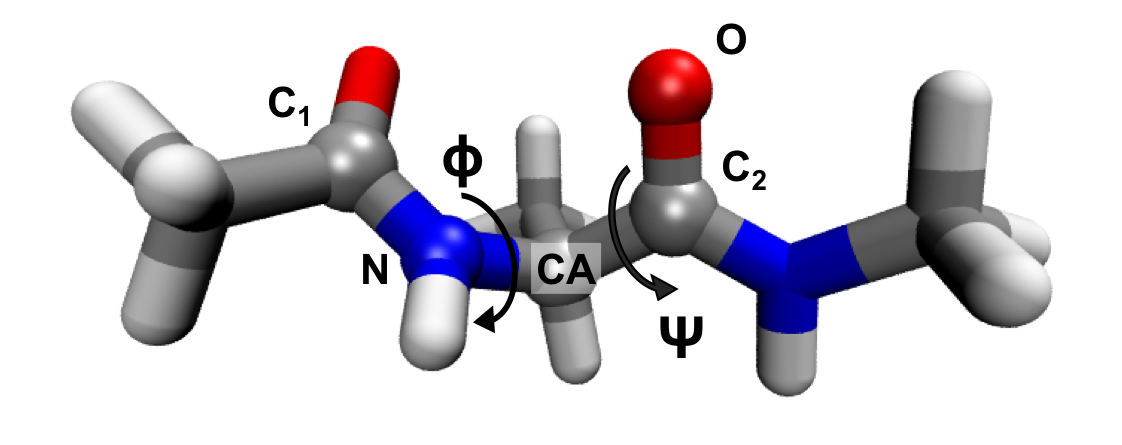
\includegraphics[width=0.8\textwidth]{chapters/msm_optimization/figures/phi_psi_ala-dp.png}
    \caption[Structure of alanine dipeptide and definition of dihedral angles]{\textsc{Structure of alanine dipeptide and definition of dihedral angles}. Grey, blue, red and white colors represent carbon, nitrogen, oxygen and hydrogen atoms respectively. The atoms involved in the $\phi, \psi$ dihedral angles are labeled and highlighted as spheres.  The $\phi$ angle is formed from the intersection of the planes formed by the atoms (C\textsubscript{1}, N, CA) and (N, CA, C\textsubscript{2}).  The $\psi$ angle is formed from the planes formed by the atoms (N, CA, C\textsubscript{2}) and (CA, C\textsubscript{2}, O).}
    \label{fig:ala1_structure}
\end{figure}

A molecular dynamics data set  of alanine dipeptide was taken from reference \cite{nuskeMarkovStateModels2017b}. This data-set has been used a benchmark for a number of molecular kinetic methods \cite{wehmeyerTimelaggedAutoencodersDeep2018a, nuskeMarkovStateModels2017b, nuskeCoarsegrainingMolecularSystems2019, wangMachineLearningCoarseGrained2019, liNeuralCanonicalTransformation2020, varolgunesInterpretableEmbeddingsMolecular2020, nuskeSpectralPropertiesEffective2021, sechiEstimationKoopmanGenerator2021, mardtVAMPnetsDeepLearning2018}. It consists of $3\times \SI{250}{\nano\second}$ trajectories sampled from a constant volume, constant temperature ensemble at $T=\SI{300}{\kelvin}$ controlled using a Langevin thermostat in explicit (TIP3P \cite{jorgensen1983comparison}) water \cite{nuskeMarkovStateModels2017b}. The sampling was performed using the ACEMD \cite{harveyACEMDAcceleratingBiomolecular2009} package, with the AMBER ff-99SB-ILDN \cite{lindorff-larsenImprovedSidechainTorsion2010} force field and a \SI{2}{\femto\second} time-step \cite{nuskeMarkovStateModels2017b}. Electrostatic forces were computed using the particle-mesh Ewald (PME) \cite{dardenParticleMeshEwald1993} summation method every two time-steps with  real-space cutoff \SI{9}{\angstrom} and grid spacing \SI{9}{\angstrom}, and all bonds to hydrogen atoms were constrained \cite{nuskeMarkovStateModels2017b}. The atomic coordinates were saved every \SI{1}{\pico\second} and the three trajectories were split into $750\times\SI{1}{\nano\second}$ smaller trajectories of \num{1000} frames each. 



\subsection{MSM fitting and scoring}\label{subsec:msm_fitting}
\begin{figure}
    \centering
    \begin{lstlisting}
estimator:
  eval: Pipeline([('cluster', 
                KmeansClustering(n_clusters=1, 
                                 max_iter=1000, 
                                 stride=10)),
                ('msm', MaximumLikelihoodMSM(lag=9, 
                                             score_k=5, 
                                             score_method='VAMP2'))])
  eval_scope: pyemma

strategy:
  name: random

search_space:
  cluster__n_clusters:
    min: 10
    max: 1000
    type: int

cv:
    name: shufflesplit
    params:
      n_splits: 20
      test_size: 0.5

dataset_loader:
  name: numpy
  params:
    filenames: *.npy

trials:
  uri: sqlite:///osprey-trials.db
  project_name: psi
    \end{lstlisting}
    \caption[Example Osprey configuration file for sampling and scoring hyperparameters]{\textsc{Example Osprey configuration file for sampling and scoring hyperparameters}. This specifies randomly sampling the number of cluster centers, clustering feature trajectories using k-means, estimating an MSM, scoring using the VAMP-2 score with 50:50 shuffle split cross-validation.}\label{fig:osprey_config}
\end{figure}

In order to  model the response surface of an MSM, a hyperparameter trial data set  $\mathcal{D} = \left\{ (\mathbf{x}_{i}, y_{i}) \right\}$ was created. This was created by  randomly sampling hyperparameters, $\mathbf{x}$, building an MSM using $\mathbf{x}$, and then measuring the MSM response, $y$, using the VAMP-2 score. 

The hyperparameter search space of alanine dipeptide is shown in table \ref{tab:ala2searchspace}. It consists of only two hyperparameters, the peptide feature, $\chi$, and the number of cluster centres, $n$.  The structure of alanine dipeptide is shown in figure \ref{fig:ala1_structure} where the two dihedral angles used as features are also labelled.  For each value of $\chi$, \num{100} values of $n$ were randomly sampled and scored. This number was chosen to ensure variation in the response with respect to $n$ was captured. A similar study \cite{husicOptimizedParameterSelection2016} used between \num{33} and \num{100} randomly sampled values per hyperparameter. This meant $\mathcal{D}$ contained $N=500$ hyperparameter trials.  

The response of each trial was measured by building an MSM with a lag time of $\tau_{\mathrm{M}} = \SI{9}{\pico\second}$ and evaluated using VAMP-2 scored with the first $r=5$ eigenvalues, in line with reference \cite{bowmanQuantitativeComparisonAlternative2013}. \num{20} iterations of 50:50 shuffle-split cross-validation, described in algorithm \ref{alg:shuffle_split}, was used when estimating the VAMP-2 score. 

The calculations for this chapter were performed in two stages: 
\begin{enumerate}
    \item \textbf{Creation of hyperparameter trial data set}: Markov state models with randomly sampled hyperparameters were estimated and scored. To manage this process the open-source software packages Osprey \cite{mcgibbonOspreyHyperparameterOptimization2016} and PyEMMA \cite{schererPyEMMASoftwarePackage2015a} were adapted by the author of this thesis.  This data was used to estimate the response surface of MSMs of alanine-dipeptide. 
    \item \textbf{Response surface estimation and Bayesian optimisation}: The response surface was estimated and Bayesian optimisation was performed also using code developed by the author of this thesis. 
\end{enumerate}
These two sets of calculations are described below. 

\subsubsection*{Creation of hyperparameter trial data set} 
The sampling of hyperparameters and fitting of MSMs was managed by a development version of Osprey (version 1.2.0dev) \cite{mcgibbonOspreyHyperparameterOptimization2016} adapted by the author of this thesis and made available on the code sharing platform GitHub (link to code repository: \href{https://github.com/RobertArbon/osprey/tree/1a108009e560b6d5e989bb2bd1555ec62e6795d0}{\color{blue}https://github.com/RobertArbon/osprey}). The main changes made were: fixing programming bugs and addition of code to allow compatibility with the package PyEMMA.  The fitting and scoring of the MSMs was performed with a development version of PyEMMA (version 2.4) \cite{schererPyEMMASoftwarePackage2015a} adapted by the author of this thesis to be compatible with Osprey, also available on GitHub (link to code repository: \href{https://github.com/RobertArbon/PyEMMA/tree/39bcb0f7b43f4424072e3e67fdff1b12cb62c99d}{\color{blue}https://github.com/RobertArbon/PyEMMA}). The main changes made were to make all the programming classes used in PyEMMA compatible with the application programming interface used by Osprey. Python version 3.5 was used throughout. 

The combination of Osprey and PyEMMA code developed here allows the user to score  maximum likelihood Markov state models using the following workflow: 
\begin{enumerate}
    \item Extract features from molecular dynamics trajectories (for example using MDTraj \cite{mcgibbonMDTrajModernOpen2015}) and store in NumPy arrays \cite{waltNumPyArrayStructure2011}.
    \item In an Osprey configuration file specify:
    \begin{enumerate}
        \item a trajectory preprocessing (e.g., TICA and clustering) and MSM estimation pipeline using the PyEMMA syntax;
        \item the method for hyperparameter sampling: random sampling, grid search, or Bayesian optimisation;
        \item the hyperparameter search space;
        \item the type of cross-validation (e.g., shuffle-split) along with the number of cross-validation iterations. 
    \end{enumerate}
    \item Osprey can then be used to sample hyperparameters, score Markov state models and store the results. 
\end{enumerate}

An example Osprey configuration file is shown in figure \ref{fig:osprey_config}.  This configuration file loads trajectories of a protein feature stored in NumPy \cite{waltNumPyArrayStructure2011} arrays (with \texttt{npy} file extension). K-means clustering is performed using the PyEMMA \texttt{KmeansClustering} class.  A maximum likelihood Markov state model is estimated using the PyEMMA class \texttt{MaximumLikelihoodMSM},  with a Markov lag time of \texttt{lag=9} frames. Model scoring is performed using the VAMP-2 score (\texttt{score\_method='VAMP2'}) with $5$ eigenvalues (\texttt{score\_k=5}). Hyperparameters are selected at random (\texttt{name: random}) by selecting the number of cluster centers (\texttt{cluster\_\_n\_clusters}) from the interval $[10, 1000]$. Cross-validation (\texttt{cv}) using the shuffle split algorithm (\texttt{name: shufflesplit}) with 20 iterations (\texttt{n\_splits: 20}) and a test-train data split of \SI{50}{\percent} (\texttt{test\_size: 0.5}).  Information on how to run Osprey can be found in the accompanying documentation, see reference \cite{mcgibbonOspreyHyperparameterOptimization2016}. 


\subsubsection*{Bayesian optimisation and analysis}
Although the Osprey code can perform Bayesian optimisation, the Bayesian optimisation and estimation of MSM response surfaces were performed separately using code developed the by author of this thesis. All code for this chapter can be found on Github (link to code repository: \href{https://github.com/RobertArbon/alanine_dipeptide/tree/fbe3ac7259e4da5cab15a60bffa9725b0b322bfd}{\color{blue}https://github.com/RobertArbon/alanine\_dipeptide}). This was written in Python 3.7 using the packages PyEMMA (version 2.5) \cite{schererPyEMMASoftwarePackage2015a}, MDTraj (version 1.9) \cite{mcgibbonMDTrajModernOpen2015}, NumPy (version 1.19) \cite{waltNumPyArrayStructure2011}, Pandas (version 0.23) \cite{mckinneyPandasFoundationalPython2011}, Matplotlib (version 3.3) \cite{hunterMatplotlib2DGraphics2007},  Seaborn (version 0.10) \cite{michaelwaskomMwaskomSeabornV02020} and the Jupyter Project (version 4.6) \cite{kluyverJupyterNotebooksPublishing2016}.

\begin{table}
    \caption[Hyperparameter search space of alanine dipeptide]{\textsc{Hyperparameter search space of alanine dipeptide}. Prior to feature selection the Cartesian coordinates of the MD trajectories were first aligned to a single, randomly chosen, trajectory frame so that features (2) and (5) did not include spurious rotational or translational motion.  The number of dimensions, `Dim.', refers to the number of individual feature variables created by $\chi$.}
    \centering
    \begin{tabularx}{0.9\textwidth}{ >{\raggedright\arraybackslash}X lll >{\raggedright\arraybackslash}X } 
    \hline
    \textbf{Hyper-parameter} & \textbf{Type} & \textbf{Range} &\textbf{Dim.} & \textbf{Details} \\
     \hline\hline
    Feature, $\chi$ & Categorical & (1) $(\phi, \psi)$ & $2$ & Torsions \\
    & & (2) (x, y, z) & $30$ & Heavy atoms only  \\
    & & (3) $\phi$ & $1$ & Torsion \\ 
    & & (4) $\psi$ & $1$ & Torsion \\ 
    & & (5) RMSD & $1$ & Heavy atoms only\\ 
    \hline 
    Cluster centres, $n$ & Integer & \numlist[list-final-separator = { ... }]{10;11;1000} & & Clustered using k-means clustering \\
     \hline
    \end{tabularx}
    \label{tab:ala2searchspace}
\end{table}

\subsection{Gaussian process regression}\label{subsec:gp}

A Gaussian process (GP) is a distribution over functions \cite{rasmussenGaussianProcessesMachine2006}.  In other words, drawing a sample from a GP return a mapping from $\mathbf{x}$, an, in general multidimensional input variable, to a continuous output variable $f(\mathbf{x})$. Considering this function at a set of discrete points, $\mathbf{x}_{1}, \mathbf{x}_{1},\ldots, \mathbf{x}_{N}$, will give a set of random variables, which together form a multivariate normal distribution: 

\begin{equation}
\begin{bmatrix}  f\left(\mathbf{x}_{1}\right) \\ \vdots \\ f\left(\mathbf{x}_{N}\right) \end{bmatrix} 
\sim 
\mathcal{N}\left( 
\begin{bmatrix} \mu\left(\mathbf{x}_{1}\right) \\  \vdots \\ \mu\left(\mathbf{x}_{N}\right) \end{bmatrix}, 
\begin{bmatrix}
k(\mathbf{x}_{1}, \mathbf{x}_{1}) & \cdots & k(\mathbf{x}_{1}, \mathbf{x}_{N}) \\
\vdots & \ddots & \vdots \\
k(\mathbf{x}_{N}, \mathbf{x}_{1}) & \cdots & k(\mathbf{x}_{N}, \mathbf{x}_{N}) \\
\end{bmatrix}
\right)\label{eqn:msm_mvn}
\end{equation}

Equation \ref{eqn:msm_mvn} is a realisation of a Gaussian process at a set of discrete input points. At each  input value, $\mathbf{x}$, there is an associated Gaussian random variable, $f(\mathbf{x})$, with a mean $\mu(\mathbf{x})$, a variance $k(\mathbf{x}, \mathbf{x})$, and a covariance between $f$ at $\mathbf{x}$ and  $\mathbf{x}^{\prime}$ given by $k(\mathbf{x}, \mathbf{x}^{\prime})$. The function $k$ is called the covariance function or \emph{kernel}.  Equation \ref{eqn:msm_mvn} can be written succinctly as $\mathbf{f} \sim \mathcal{N}(\bm{\mu}, \mathbf{K})$ \cite{rasmussenGaussianProcessesMachine2006}. A salient example\footnote{this example is used in reference \cite{rasmussenGaussianProcessesMachine2006} and is the `hello world' example of GP regression modelling, frequently used in other texts and probabilistic programming tutorials e.g., reference \cite{salvatierProbabilisticProgrammingPython2016}} is that of daily atmospheric carbon dioxide levels at the Mauna Loa observatory.  $\mathbf{x} = x$ is a variable representing time (measurements are daily) while $f(x)$ are the daily carbon dioxide levels. The levels rise and fall over the course of the year meaning daily measurements are correlated and this is captured in the function $k(x, x^{\prime})$.  A GP can be subject to some random additive noise, $\epsilon$,  then this is written $y = f(\mathbf{x}) + \epsilon$. This can also be written as $\mathbf{y} \sim \mathcal{N}(\mathbf{f}, \sigma_{n}^{2}\mathbf{I})$, where $\mathbf{I}$ is the identity matrix and $\sigma_{n}^{2}$ is the variance of the noise \cite{rasmussenGaussianProcessesMachine2006} (the mean of the noise is assumed to be zero).  Continuing the example, $\epsilon$, would represent random errors in the measurement of carbon dioxide levels. 

% So far a GP is just a probability distribution over functions, $\mathbb{P}(\mathbf{f})$, independent of observed data. In order to make draws from this distribution the mean function and kernel must be specified.
In order to make the link between the theoretical construct of a GP (equation \ref{eqn:msm_mvn}) and modelling data, two ingredients are needed: a kernel function $k(\mathbf{x}, \mathbf{x}^{\prime})$ and method of incorporating observations, $(\mathbf{x}_{i}, y_{i})$, $i = 1 - N$, where $N$ is the number of observations.  To center this discussion consider the Gaussian kernel \cite{rasmussenGaussianProcessesMachine2006}: 
\begin{equation}\label{eqn:eg_rbf}
    k(\mathbf{x}, \mathbf{x}^{\prime}) = \exp{\left(-\frac{\left|\mathbf{x}-\mathbf{x}^{\prime}\right|^{2}}{l^{2}}\right)}
\end{equation}\label{eqn:msm_rbf}
This states that values of the GP will be highly correlated between values of $\mathbf{x}$ that are `similar' and less correlated when they are separated. The value of $l$ is the characteristic length-scale of the GP and determines how close values of $\mathbf{x}$ must be to be considered `similar' \cite{rasmussenGaussianProcessesMachine2006}. In other words, it determines how rapidly  $y$ changes for changes in $\mathbf{x}$. 

The process of fitting a GP model, $\mathbf{y} \sim \mathcal{N}(\mathbf{f}, \sigma_{n}^{2}\mathbf{I})$, using a Gaussian kernel in the definition of $\mathbf{f}$ (equation \ref{eqn:eg_rbf}), can be thought of as: 
\begin{enumerate}
    \item choosing values of $\mu(\mathbf{x}_{i})$,
    \item a value of $l$, which in turn completely defines $k(\mathbf{x}, \mathbf{x}^{\prime})$ (this is a kernel hyperparameter), and
    \item and a value the variance of $\sigma_{n}$, 
\end{enumerate}  
which are consistent with the training data $\mathcal{D}=\left\{(\mathbf{x}_{i}, y_{i})\right\} = (\mathbf{y}, \mathbf{X})$ and all prior knowledge of the system. In order to do this,  Bayes' rule is used \cite{rasmussenGaussianProcessesMachine2006}:
\begin{equation}\label{eqn:ya_boy_bayes}
    \mathbb{P}(\mathbf{f}|\mathbf{y}, \mathbf{X})  = \frac{\mathbb{P}(\mathbf{y}|\mathbf{f}, \mathbf{X})\mathbb{P}(\mathbf{f})}{\mathbb{P}(\mathbf{y}|\mathbf{x})}. 
\end{equation}
The posterior distribution $\mathbb{P}(\mathbf{f}|\mathbf{y}, \mathbf{X})$ is the distribution over all possible GPs, $\mathbf{f}$, which are consistent \emph{with the training data} $(\mathbf{y}, \mathbf{X})$. In other words, draws from this distribution will now (hopefully) resemble the data. The posterior takes into account the training data  through the likelihood function $\mathbb{P}(\mathbf{y}|\mathbf{f}, \mathbf{X}) = \mathcal{N}(\mathbf{f}, \sigma_{n}^{2}\mathbf{I})$. This is the probability of observing the outputs, \emph{given the inputs and a specific GP}, $\mathbf{X}$ and $\mathbf{f}$.  The term $\mathbb{P}(\mathbf{f})$ is a probability distribution over all possible functions $\mathbf{f}$, it incorporates all previous knowledge of the system being studied and is known as the prior \cite{gelmanBayesianDataAnalysis2014}.  In practice this amounts to specifying a value of $\mu(\mathbf{x})$ and in the current example, a distribution of different values of $l$.  If nothing is known about the system, a value of $\mu(\mathbf{x})=0$ and a wide distribution of values over $l$ would be appropriate. In effect this would mean both highly correlated and weakly correlated GPs are both \emph{a priori}, likely\cite{gelmanBayesianDataAnalysis2014}.  The term $\mathbb{P}(\mathbf{y}|\mathbf{x})$  a factor for normalizing the posterior distribution. 

The posterior distribution is also a GP and can be written as follows.  Let $\bar{f}_{*}$ be the mean of the posterior GP at some arbitrary point $\mathbf{x}_{*}$ (which may or may not be in the training data), and let $\mathbb{V}\left[f\right]$ be the covariance between value of the GP at this point and all other points in the training data, then \cite{rasmussenGaussianProcessesMachine2006}:
\begin{equation}\label{eqn:gp_pred_dist}
\begin{aligned}
\bar{f}_{*} &=\mathbf{k}_{*}^{\top}\left(\mathbf{K}+\sigma_{n}^{2} \mathbf{I}\right)^{-1} \mathbf{y} \\
\mathbb{V}\left[f_{*}\right] &=k\left(\mathbf{x}_{*}, \mathbf{x}_{*}\right)-\mathbf{k}_{*}^{\top}\left(\mathbf{K}+\sigma_{n}^{2} \mathbf{I}\right)^{-1} \mathbf{k}_{*}.
\end{aligned}
\end{equation}
Here $\mathbf{k}_{*}$ is a vector of covariances between $\mathbf{x}_{*}$ and the training observations, $\mathbf{X}$. As the point $\mathbf{x}_{*}$ is arbitrary, these equations define the posterior GP over the entire domain. 

Equations \ref{eqn:gp_pred_dist} only determine how the posterior GP should be defined in terms of the training data and the hyperparameters\footnote{not to be confused with the hyperparameters of the MSM which are the predictors of the GP.} of the kernel function, e.g., $l$ in equation \ref{eqn:eg_rbf}.  Kernel hyperparameters can be estimated from the data using Bayesian estimation or by maximizing the \emph{log marginal likelihood} \cite{rasmussenGaussianProcessesMachine2006}:
\begin{equation}\label{eqn:marg_llike}
\log{\left( \mathbb{P}(\mathbf{y} | \mathbf{X})\right)}=-\frac{1}{2} \mathbf{y}^{\top}\left(\mathbf{K}+\sigma^{2} \mathbf{I}\right)^{-1} \mathbf{y}-\frac{1}{2} \log \left|\mathbf{K}+\sigma^{2} \mathbf{I}\right|-\frac{N}{2} \log 2 \pi.
\end{equation}
The values of the kernel hyperparameters estimated by maximizing the log marginal likelihood, equation \ref{eqn:marg_llike} are known as maximum \emph{a posteriori} (MAP) estimates \cite{rasmussenGaussianProcessesMachine2006}. These are single point estimates of the kernel hyperparameters. When estimates of variability of kernel hyperparameters are required, Bayesian estimation can be used \cite{gelmanBayesianDataAnalysis2014}. In this case Markov chain Monte Carlo (MCMC) is used to sample the posterior distribution of $l$. The same considerations for Bayesian MSMs in section \ref{sec:theory_bayes} apply in this case. 

The process of fitting a GP to data can be summarised as follows:
\begin{enumerate}
    \item collect training data $\mathcal{D}$, 
    \item specify a prior mean function, 
    \item  specify a functional form of covariance kernel $k(\mathbf{x}, \mathbf{x}^{\prime})$, e.g., equation \ref{eqn:eg_rbf}, 
    \item specify priors over the kernel hyperparameters, 
    \item fit the GP by maximizing the log marginal likelihood, equation \ref{eqn:marg_llike} or using Bayesian estimation. 
\end{enumerate}

\subsection{Evaluating model fit}\label{subsec:gp_fit}

There is considerable flexibility when using GPs to model data. First, there is a wide variety of kernels that can be used, see for example reference \cite{duvenaudAutomaticModelConstruction2014} which presents a `cook-book' for constructing complex kernels from other kernels. The input variables may also be transformed, a process known as input warping \cite{snoekInputWarpingBayesian2014a}, e.g., a logarithmic warping would be to replace $x \rightarrow \log{(x)}$. 

A method for evaluating a comparing GPs constructed with different kernels and input warpings is needed. For models fit by maximizing the marginal likelihood the predictive value of the GP can be measured through the standardized mean square error (SMSE) and the mean standardized log loss (MSLL) \cite{rasmussenGaussianProcessesMachine2006}. These play the same r\^ole as, for example, the $R^2$ or deviance play in generalized linear models \cite{dobson2018introduction}. The SMSE is defined by \cite{rasmussenGaussianProcessesMachine2006}:
\begin{equation}\label{eqn:smse}
\mathrm{SMSE} =\left(\frac{1}{N}\right) \mathlarger{\mathlarger{\sum}}_{i=1}^{N} \frac{\left(f(x)-y_{i}\right)^{2}}{\sigma_{obs}^{2}},
\end{equation}
and the mean standardized log loss (MSLL) by \cite{rasmussenGaussianProcessesMachine2006}:
\begin{equation}\label{eqn:msll}
\mathrm{MSLL}=\left(\frac{1}{N}\right) \mathlarger{\mathlarger{\sum}}_{i=1}^{N}\left[\left(\frac{1}{2} \log \left(2 \pi \sigma_{i}^{2}\right)+\frac{\left(f(x)-y_{i}\right)^{2}}{2\sigma_{i}^{2}}\right)-\left(\frac{1}{2} \log \left(2 \pi \sigma_{obs}^{2}\right)+\frac{\left(\bar{y}-y_{i}\right)^{2}}{2\sigma_{obs}^{2}}\right)\right].
\end{equation}  

\begin{figure}
    \centering
    \caption[Mean standardized log-loss (MSLL) and standardized mean square error (SMSE)]{\textsc{Mean standardized log-loss (MSLL) and standardized mean square error (SMSE)}. Panels (a) - (c) show three different GPs fit to the same data after 3, 6, 9 steps, respectively, of marginal likelihood maximization. The MSLL and SMSE is for each GP is labelled. The blue line and shaded blue area are the mean and uncertainty of the GP, the black crosses are the observations, and the dashed and dotted lines are the mean and uncertainty of the null model (i.e., mean and uncertainty of $y_{i}$).}
    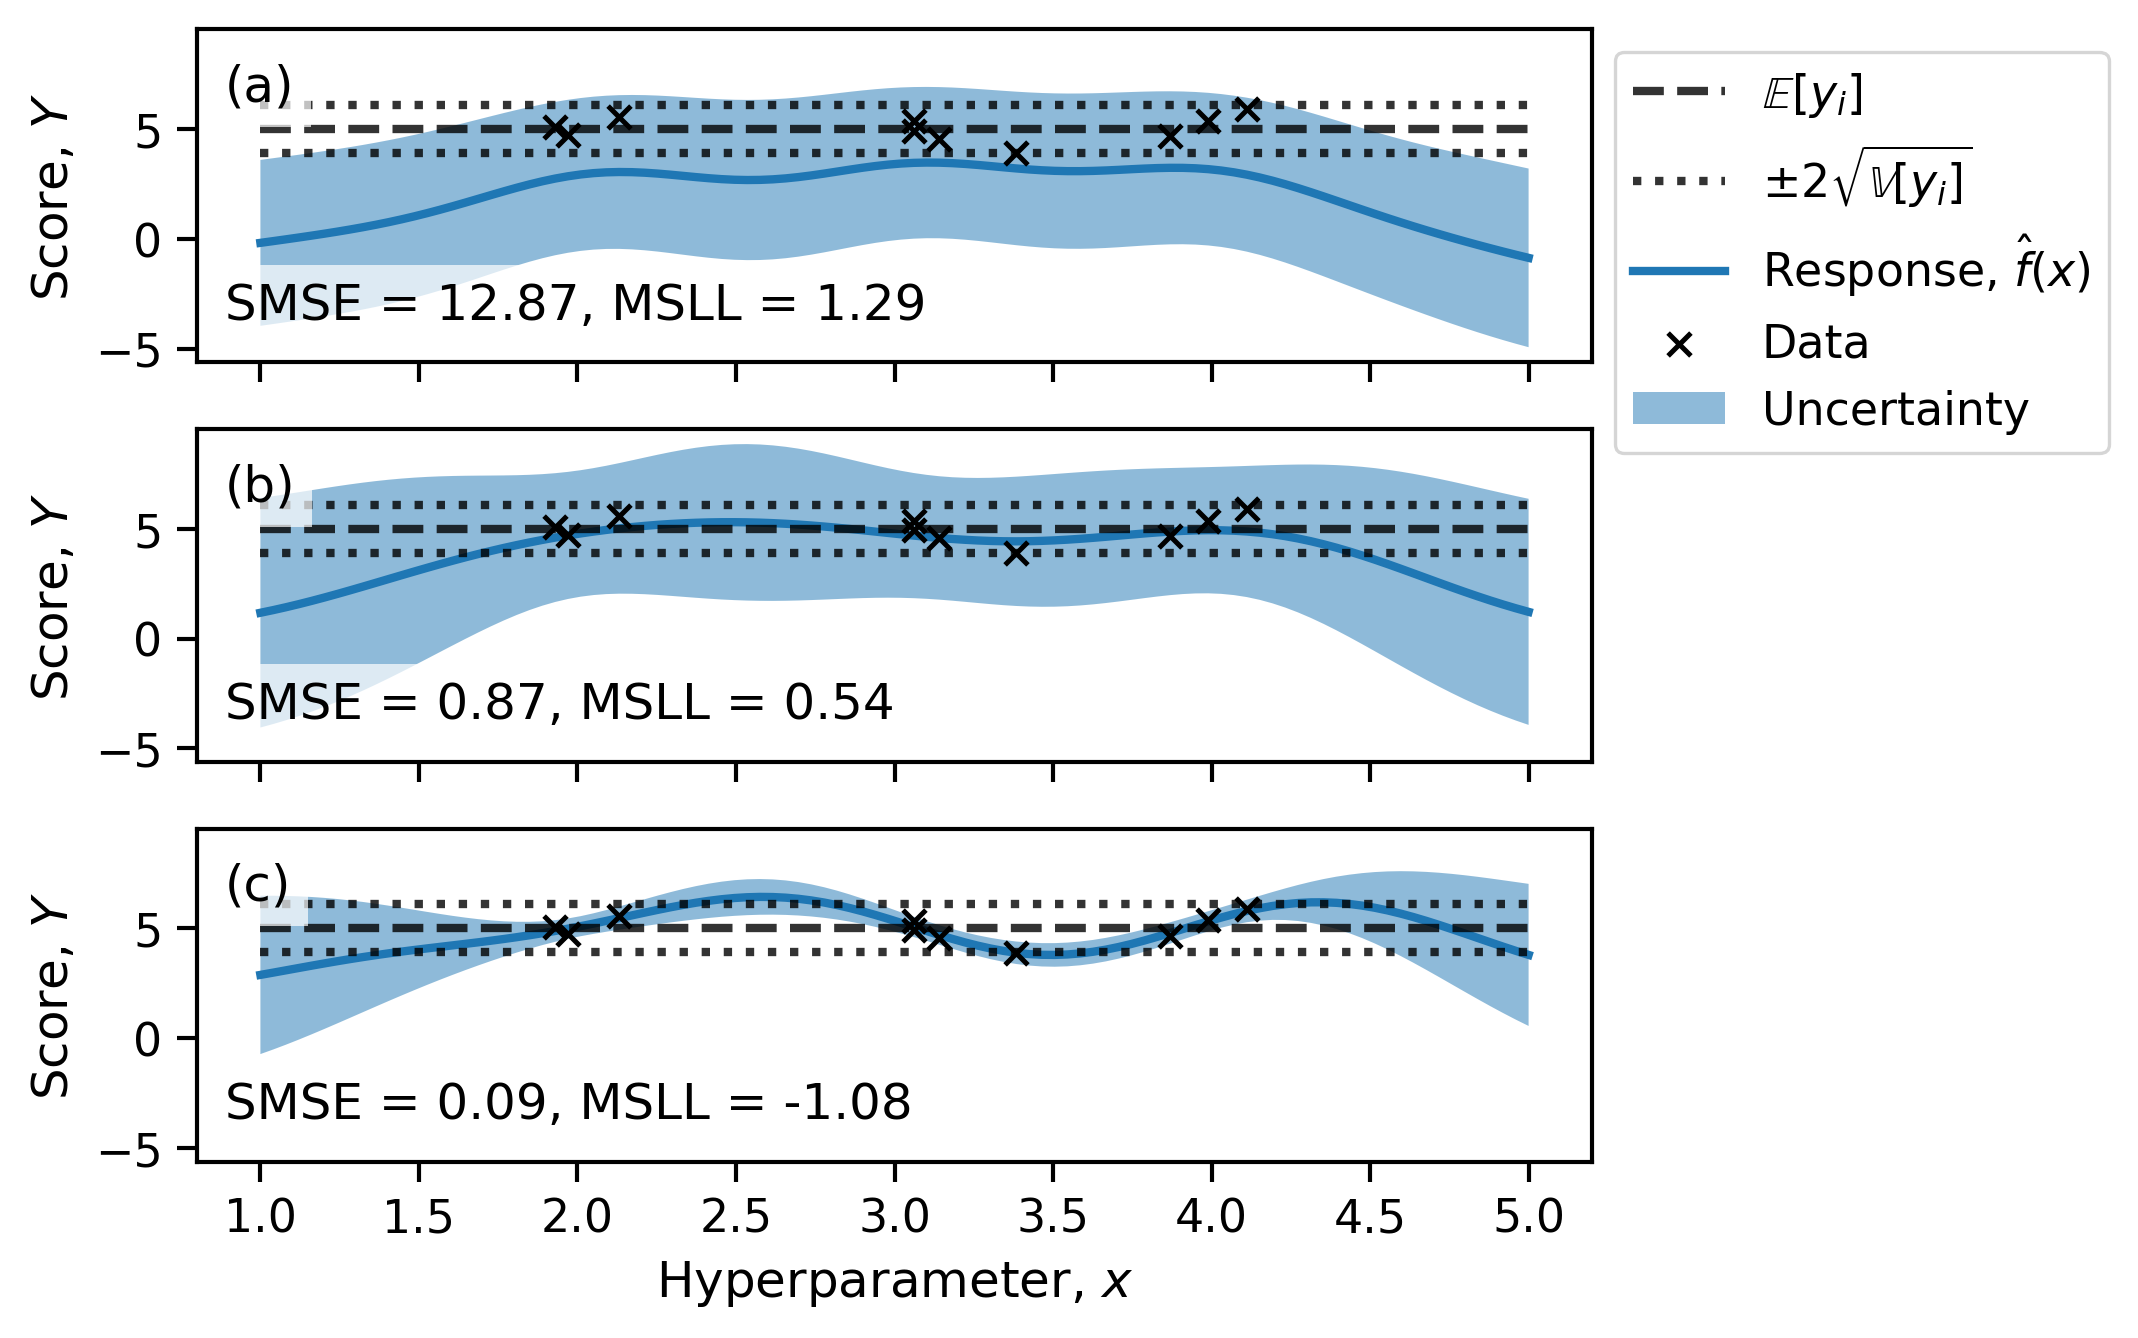
\includegraphics[width=0.8\textwidth]{chapters/msm_optimization/figures/gp_metric_explainer.png}
    \label{fig:msm_gp_metric_explainer}
\end{figure}

Here $\sigma_{obs}^{2}$ is the observed variance of the training data response, $\mathbb{E}\left[(y_{i}-\bar{y})^{2}\right]$, and $\sigma_{i}^{2}$ refers to the GP predicted variance at the observation $i$ including the noise term (i.e., $\mathbb{V}\left[f_{*}\right]+\sigma_{n}^{2}$, from equation \ref{eqn:gp_pred_dist}).  The `standardization' in each case is to allow both metrics to compare the fitted GP to a null model which simply predicts the mean and variance of the observed $y_{i}$ at each value of $\mathbf{x}_{i}$ i.e., \cite{rasmussenGaussianProcessesMachine2006}:
\begin{equation}\label{eqn:gp_null}
\begin{aligned}
\bar{f}^{\mathrm{Null}}_{*} &= \mathbb{E}\left[y_{i}\right] \\
\mathbb{V}^{\mathrm{Null}}\left[f_{*}\right] &= \mathbb{V}\left[y_{i}\right].
\end{aligned}
\end{equation}

To gain intuition of the SMSE and MSLL consider figure \ref{fig:msm_gp_metric_explainer}. Panels (a), (b) and (c) show a GP fit to the same data as figure \ref{fig:msm_rsm_explainer} after 3, 6, and 9 iterations of marginal likelihood maximization. This would not be done in practice but serves as an example of three models which differ in how well they fit the data. In practice these differences would arise from different kernels etc. The null model is denoted by the dashed and dotted lines (mean and uncertainty respectively), while the mean and the uncertainty in the fitted GP are denoted by the blue line and shaded blue area respectively.  In panel (a) the fitted GP is clearly worse than predicting the mean of the observations, so  $\mathrm{SMSE} > 1$ and  $\mathrm{MSLL} > 0$. In panel (b) the GP fits the data well so $\mathrm{SMSE} < 1$ but the variance of the GP is still much larger than the variance of the observations so $\mathrm{MSLL} > 0$. In panel (c) the GP fits the observations almost exactly so $\mathrm{SMSE} \simeq 0$, and the variance of the GP at each observed $\mathbf{x}_{i}$ is smaller than variance of the observations so $\mathrm{MSLL} < 0$. 

In this thesis, the MSLL and SMSE were estimated using K-fold cross-validation \cite{friedman2001elements} to avoid choosing a kernel or input warping which may over-fit to a particular data set. The K-fold cross-validation procedure is as follows \cite{friedman2001elements}: first split the hyperparameter trial data set, $\mathcal{D},$ into a $K$ equally sized, disjoint, sets or `folds'. Second, fit the GP using $K-1$ folds and then calculate the SMSE and MSLL on the remaining $1$ fold. Third, repeat this process $K$ times, training the GP and calculating the SMSE and MSLL with a different held out fold each time. The cross-validated MSLL and SMSE is the weighted mean of the SMSE and MSLL on each fold. 

\subsection{Response surface modelling}\label{subsec:rsm}
The VAMP-2 response of the MSM with respect to its hyperparameters, $\mathbf{x} = (\chi, n)$, was modelled as a GP with additive noise. A variety of combinations of input warping (e.g., log-transformation of $\mathbf{x}$) and covariance kernels, $k(\mathbf{x}, \mathbf{x}^{\prime})$,  were tried and the best combinations for each response surface determined using the cross-validated SMSE and MSLL. 

To reduce the computational effort required to fit each GP model, a sparse approximation to the full covariance matrix of the GP, called the fully independent training conditional (FITC) was used \cite{quinonero-candelaUnifyingViewSparse2005}. In this approximation a number of observations must be designated as `inducing points'. Larger numbers of inducing points increases the accuracy of the approximation at the expense of increased computational effort. The number of inducing points was set to $\SI{10}{\percent}$ of the total number of observations and their location determined by k-means clustering as suggested in the probabilistic programming package PyMC3 (version 3.5) \cite{salvatierProbabilisticProgrammingPython2016}. This fraction was chosen by fitting a single GP model with the number of inducing points ranging from \SI{10}{\percent} to \SI{100}{\percent} of the total observations. The number of inducing points was not found to change the posterior distribution significantly and so the smallest value was used. 

As described in the previous section, in order to fit a GP model a number of modelling choices need to specified, these are: 
\begin{enumerate}
    \item the prior of the mean function, $\mu(\mathbf{x})$;
    \item the kernel function, $k(\mathbf{x}, \mathbf{x}^{\prime})$;
    \item the prior distributions of kernel hyperparameters;
    \item the warpings of the predictors.
\end{enumerate}

The kernel function and input warping will be chosen by fitting models and selecting the combination which best fits the data. The Mean function and prior distributions over kernel hyperparameters will be set based on other consideration.

\subsubsection*{Mean function and kernel function}

The prior of mean function  was set to zero everywhere: $\mu(\mathbf{x})=\mathbf{0}$, in practice this does not have much impact on the final model \cite{brochuTutorialBayesianOptimization2010}. 

The kernel functions considered were restricted to stationary kernels, i.e., those where $k(\mathbf{x}, \mathbf{x}^{\prime}) = k(|\mathbf{x} - \mathbf{x}^{\prime}|)$. Stationary kernels are advantageous because they admit a useful interpretation of the kernel hyperparameters which will be described in section \ref{subsubsec:ala_relevance}. Mathematically they mean that the correlations between values of $y$ do not depend on the absolute values of $\mathbf{x}$ only on the distance between $\mathbf{x}$ and $\mathbf{x}^{\prime}$.
The form of kernel used in this work is the same as the one used by authors of reference  \cite{bergstrajamesbergstraRandomSearchHyperParameter2012} in their work on random search and the relevance of hyperparameters discussed in the introduction: 
\begin{equation}\label{eqn:kernel_form}
    k\left(\left|\mathbf{x}-\mathbf{x}^{\prime}\right|; \theta\right) = 
    \eta^{2}\mathlarger{\prod}_i k_{M}\left(\left|x_{i}-x_{i}^{\prime}\right|; \nu, l_i\right)
    +\sigma_{n}^{2}\delta_{\mathbf{x}, \mathbf{x}^{\prime}}. 
\end{equation}
The $\eta$ terms controls the total variation in the response function, the larger the value of $\eta$ the more the response is able vary over the whole predictor space \cite{rasmussenGaussianProcessesMachine2006}. The $\sigma_{n}^{2}$ term is the noise \cite{rasmussenGaussianProcessesMachine2006} term which allows the GP to account for variation in the response due to measurement error, which in this case amounts to variation due to the cross validation procedure.  The index, $i$, runs over each component of $\mathbf{x}$ so that $x_{i}$ refers to a single hyperparameter, e.g., $n$. The total kernel is the product of kernels over each hyperparameter.  The $M$ in $k_{M}$ denotes a Mat\'ern kernel parameterized by $\nu$ - this will be discussed below. $l_{i}$ is the characteristic length-scale of $k_{M}$. $\eta$, $\sigma_{n}$ and the $l_{i}$'s are estimated from the data and are the kernel hyperparameters, collectively denoted by $\theta$. The multiplicative form of this kernel means that VAMP-2 responses are correlated only when the values of the predictors are simultaneously similar, where the similarity is set by $l_{i}$.    

The kernels over the individual predictors were kernels in the Mat\'{e}rn class with values of $\nu=\sfrac{1}{2},\ \sfrac{3}{2},\ \sfrac{5}{2},\ \infty$. These are alternatively known as an exponential, Mat\'{e}rn 3-2, Mat\'{e}rn 5-2 and  Gaussian (Radial Basis Function, RBF) kernels.  These kernels were chosen based on their common usage \cite{shahriariTakingHumanOut2016} and  range from `rough' exponential kernel, where correlation in the response drops off rapidly with changes in the predictors, to smooth processes with the Gaussian kernel. They are defined as follows \cite{rasmussenGaussianProcessesMachine2006}: 
\begin{align}
k_{\text{Exp}}\left(r; \sfrac{1}{2}\right) &=\exp (-r) \label{eqn:kern_exp}\\
k_{\text{M3-2}}\left(r; \sfrac{3}{2}\right) &= \exp (-\sqrt{3} r)(1+\sqrt{3} r) \label{eqn:kern_m32} \\
k_{\text{M5-2}}\left(r; \sfrac{5}{2}\right) &= \exp (-\sqrt{5} r)\left(1+\sqrt{5} r+\frac{5}{3} r^{2}\right) \label{eqn:kern_m52}\\
k_{\text{RBF}}\left(r; \infty\right) &= \exp \left(-\frac{1}{2} r^{2}\right) \label{eqn:kern_gauss}
\end{align}
where $r = \frac{|x-x^{\prime}|}{l}$. See chapter 5 of  reference \cite{rasmussenGaussianProcessesMachine2006} for a full description of the Mat\'{e}rn kernels and their properties.  

\begin{figure}
    \centering
    \caption[Kernel hyperparameter priors and representative GPs]{\textsc{Kernel hyperparameter priors and representative GPs}. Panel (a) shows the prior used for the variance parameters, $\eta$, $\sigma_n$: the half-Cauchy with $\beta=2$. Panel (b) shows the prior used for the length-scale parameters $l_{i}$: the Gamma distribution with $\alpha=1, \beta=0.05$.  Panel (c) shows 10 draws from a Gaussian process with an RBF kernel (equation \ref{eqn:kern_gauss}) with values of $l$ drawn from the distribution in panel (b) and values of $\eta$ drawn from distribution in panel (a).}
    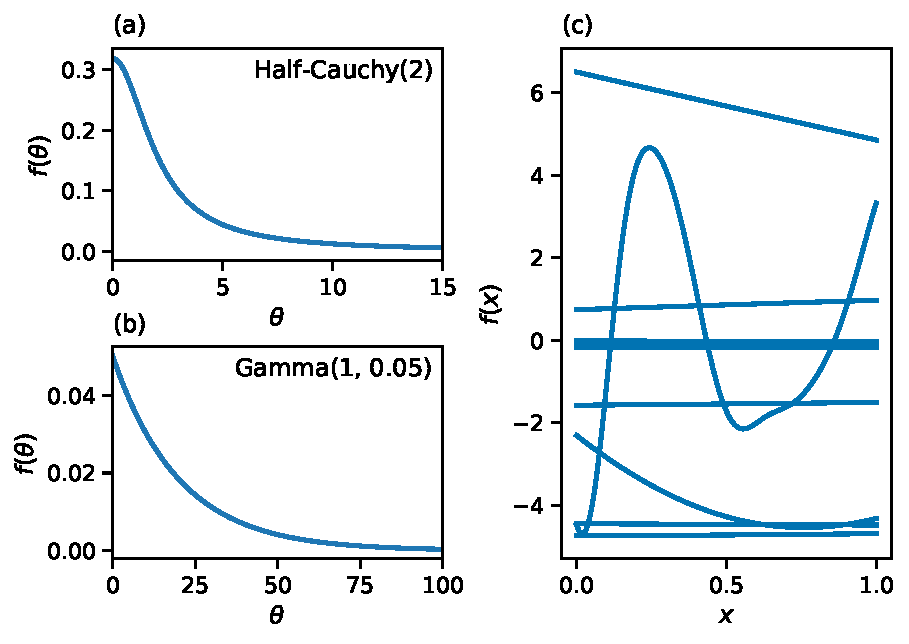
\includegraphics[width=0.8\textwidth]{chapters/msm_optimization/figures/prior_functions.pdf}
    \label{fig:priors}
\end{figure}

\subsubsection{Prior distributions of kernel hyperparameters}

Prior distributions of kernel hyperparameters affect the range of possible values  which can be estimated from the data. They serve the purpose of ensuring that the learned hyperparameters fit with prior expectations about their true values \cite{gelmanBayesianDataAnalysis2014}. 

The GP hyperparameters estimated from the data are the mean function, $\mu(\mathbf{x})$ and the kernel hyperparameters, $\theta = (\eta, \sigma_{n}, l_{1}, l_{2}, ...)$. These were estimated differently depending on the application. When the GP was used for visualisation (e.g., figure \ref{fig:ala1_response}) or for Bayesian optimisation (section \ref{sec:ala_opt}) the hyperparameters were estimated by maximizing the log marginal likelihood. When error estimates of the GP hyperparameters were needed for discussing the relevance (section \ref{subsubsec:ala_relevance}) Bayesian estimation was used. 

The prior distributions for the variance terms, $\eta$ and $\sigma_{n}$, were $\mathrm{half-Cauchy}(\beta=2)$ and the priors for the length-scale parameters, $l_{i}$, were $\mathrm{Gamma}(\alpha=1, \beta=0.05)$. These distributions are shown in figure \ref{fig:priors} panels (a) and (b) respectively.  To get a sense of the effect of these priors on a GP, 10 draws from a 1D Gaussian process with an RBF kernel are shown in  \ref{fig:priors} panel (c). The values of the $\eta$ and $l$ hyperparameters in this GP are drawn the distributions in panels (a) and (b) respectively.  

The r\^ole of weakly informative priors is to exclude unrealistic or disallowed values of the parameters without imposing strong prior beliefs on the true values \cite{gelmanBayesianDataAnalysis2014}. The half-Cauchy distribution  was used for $\eta$ and $\sigma_n$  based on its recommended use in other settings \cite{polsonHalfCauchyPriorGlobal2012}. It was only necessary for the scale of this distribution to give significant density in the range $0-5$ as the VAMP-2 score will lie in the range $[1,5]$ for alanine dipeptide thus limiting the possible values of $\eta$ and $\sigma_{n}$. The prior for $l$ was justified on the basis that, after scaling the predictors to lie in $[0, 1]$, values of $l \gg 1$ imply a flat response, meaning significant density for $l \gg 1$ is not necessary. 

\begin{figure}
    \centering
    \caption[Input warping]{\textsc{Input warping}. Panel (a) shows a non-stationary function $y$ as a function of a predictor $x$. The characteristic length-scale decreases as $x$ increases. Panel (b) shows a warping function which transforms $x$ to $x^\mathrm{W}$. Applying this warping results in the new function in panel (c) which is approximately stationary. This figure is an adaption of figure 1 in reference \cite{snoekInputWarpingBayesian2014a}.}
    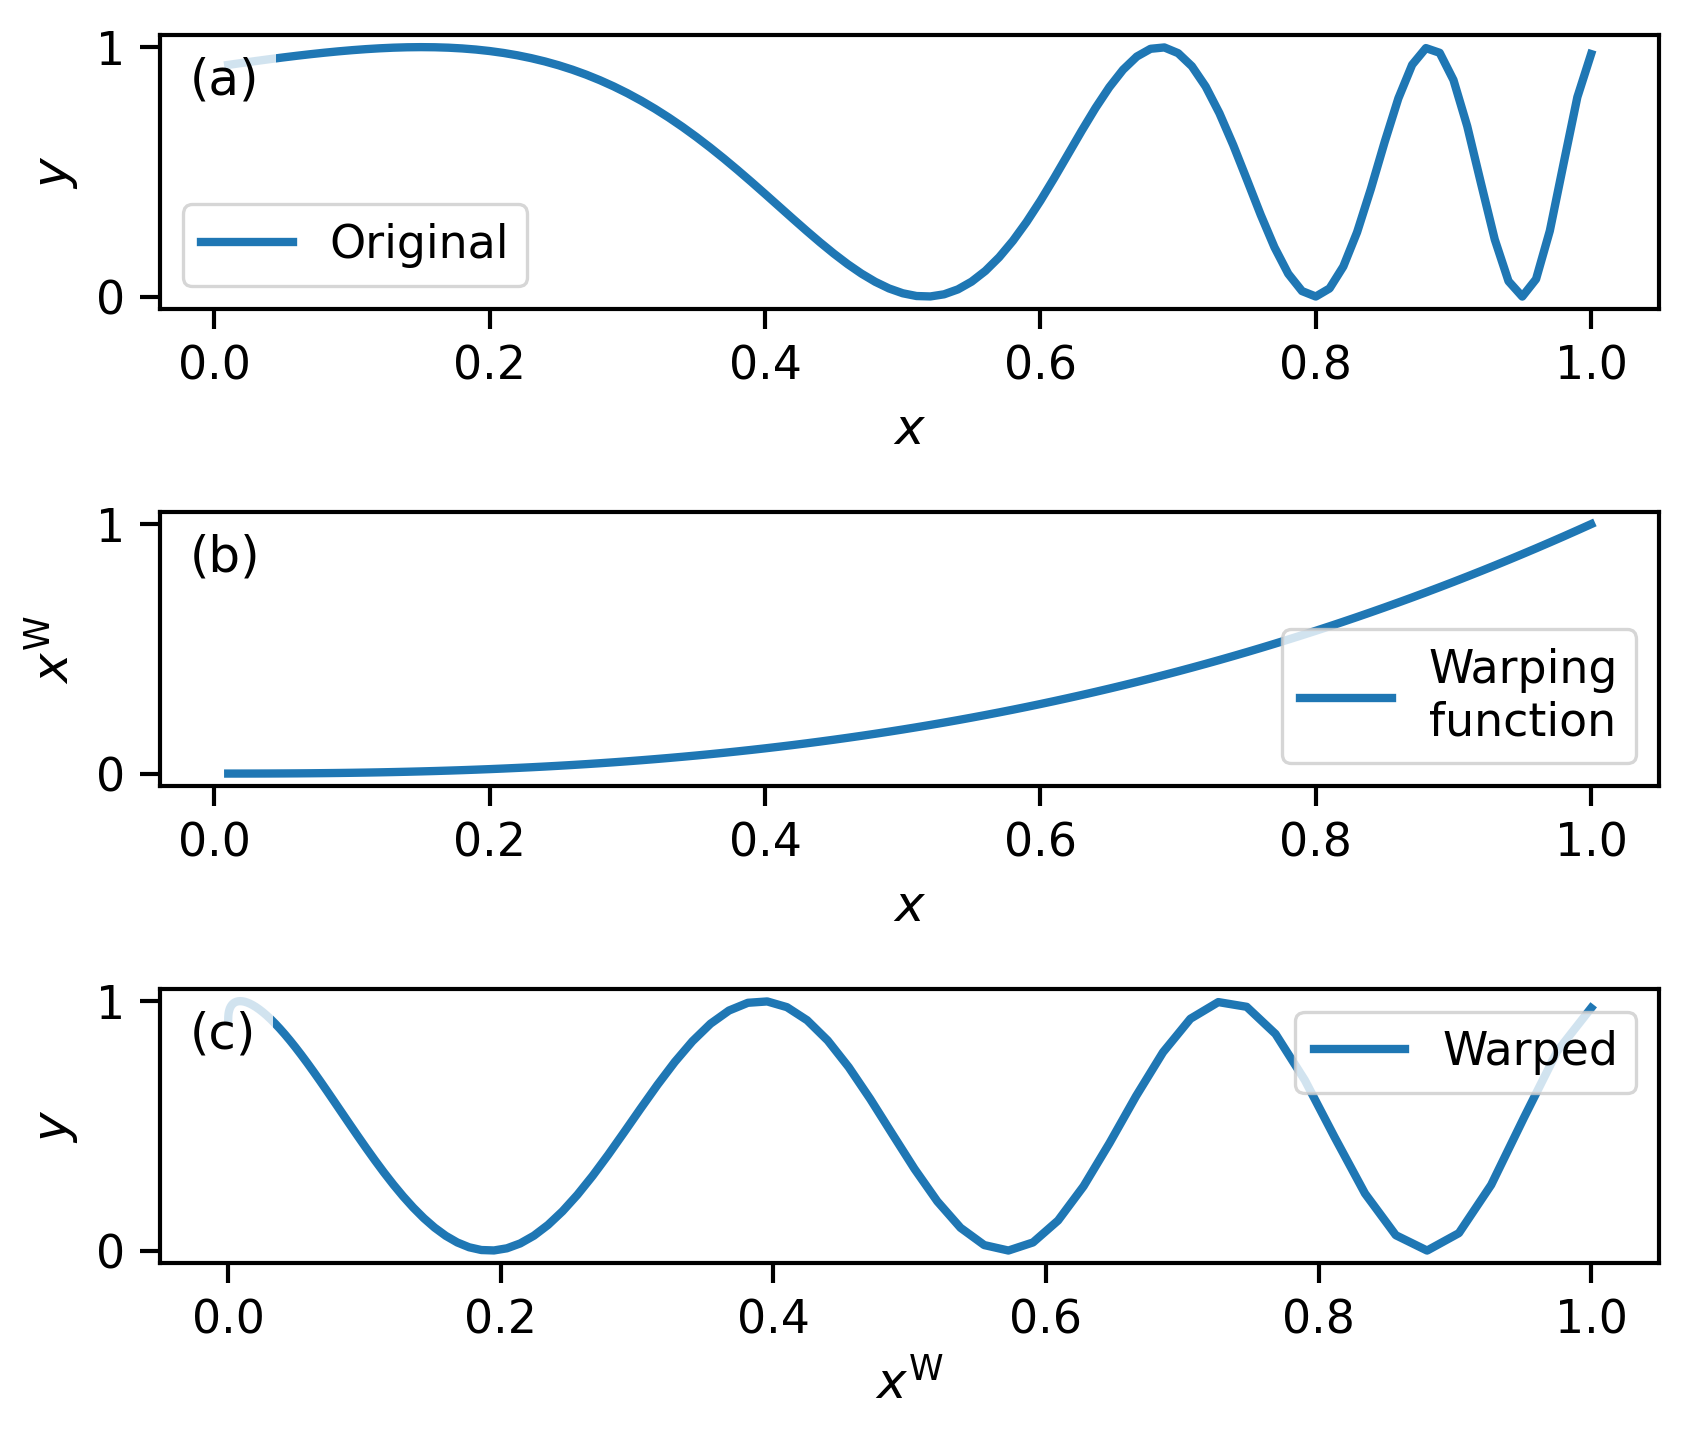
\includegraphics[width=0.8\textwidth]{chapters/msm_optimization/figures/warping_explainer.png}
    \label{fig:msm_warping_explainer}
\end{figure}

\subsubsection*{Input warpings}

The predictors were transformed in three ways: scaling,  input warping, and coding (for categorical predictors only). All predictors were scaled to lie in the range $[0, 1]$ to make the kernel length-scale parameters, $l$, comparable across different hyperparameters. Input warping is used to mitigate the problems of modelling non-stationary functions using stationary GP kernels \cite{snoekInputWarpingBayesian2014a}. Assuming stationarity i.e., that the GP characteristic length-scale  does not vary with the input $\mathbf{x}$, simplifies both estimation and interpretation of the GP \cite{snoekInputWarpingBayesian2014a}. Thus, warping predictors to make the stationarity assumption more plausible is important, especially when it comes to discussing hyperparameter relevance in section \ref{sub:msm_meth_rel}. Coding is used to transform non-numerical predictors (i.e., the protein feature) into numerical variables. 

To aide understanding of input warping, a dramatic example is shown in figure \ref{fig:msm_warping_explainer} (which is an adaption of figure 1 in reference \cite{snoekInputWarpingBayesian2014a}). Panel (a) shows a non-stationary function - the characteristic length-scale decreases with increasing $x$. In other words, the kernel function, $k(x, x^{\prime})$ could not be written as a function of $|x-x^{\prime}|$. Panel (b) shows a warping function which transforms $x$ to $x^{\mathrm{w}}$. Panel (c) applies this warping and the resultant function is more plausibly stationary. With respect to this work, two input warpings, $T(x)$, were considered: the identity $I(x)$, and a logarithmic transformation, $\log(x)$.  

The categorical predictor, $\chi$, was dummy coded \cite{dalyDummyCodingVs2016} to give a five dimensional vector of $1$s and $0$s.  A example of the transformations of two hyperparameters, $\chi$ and $n$, in preparation for modelling with a GP are shown in figure \ref{fig:msm_eg_transform}. 

\begin{figure}
    \centering
    \caption[Example predictor transformation]{\textsc{Example predictor transformation}. The left hand table shows the raw values of the hyperparameters, $\chi$ and $n$, as a data matrix. The right hand table shows same values after dummy coding $\chi \rightarrow \chi_{1}, \chi_{2}, \ldots$ and scaling $n\rightarrow n^{\mathrm{s}}$ to lie in the range $[0, 1]$. No warping was applied. The dummy coding and scaling is performed with reference to the hyperparameter search space in table \ref{tab:ala2searchspace}.}
    \begin{tabular}{cc}
        \toprule
        $\chi$    &  $n$ \\
        \midrule
        $(\phi, \psi)$    &  10 \\
        $(x, y, z)$ & 500 \\
        $\psi$  & 1000 \\
        \bottomrule
        \end{tabular}
    $\longrightarrow $
    \begin{tabular}{cccccc}
        \toprule
        $\chi_{1}$ &$\chi_{2}$ &$\chi_{3}$ &$\chi_{4}$ &$\chi_{5}$ &  $n^{\mathrm{s}}$ \\
        \midrule
        1 & 0 & 0 & 0 & 0  &  \num{0.00} \\
        0 & 1 & 0 & 0 & 0  &  \num{0.49} \\
        0 & 0 & 0 & 1 & 0  &  \num{1.00} \\
        \bottomrule
    \end{tabular} 
    \label{fig:msm_eg_transform}
\end{figure}

In order to select the best combination of kernel functions and predictor warping each possible combination was used to estimate a GP which was then evaluated using the cross-validated MSLL and SMSE. So, for the response surface of alanine dipeptide eight different models were estimated: four different types of kernel (equations \ref{eqn:kern_exp} - \ref{eqn:kern_gauss}) were used in equation \ref{eqn:kernel_form} and two predictor warpings for $n$. For each model both metrics were calculated using 10-fold cross validation. Any model with MSLL$ > 0$ or SMSE$ > 1$ was discarded. The remaining models were ranked separately according to MSLL and SMSE ($R_{\mathrm{MSLL}}$, $R_{\mathrm{SMSE}}$) and the ranks combined according to $\sqrt{R_{\mathrm{MSLL}}^2 + R_{\mathrm{SMSE}}^2}$. This ranking method was used to ensure a balance between the two selection metrics compared to, say, the mean of the two ranks.  

All GPR modelling was performed with the Python package PyMC3 (verion 3.5) \cite{salvatierProbabilisticProgrammingPython2016} with some visualisation performed using package GPy (version 1.5) \cite{gpy2014}. 

\subsection{Hyperparameter relevance}\label{sub:msm_meth_rel}

The sensitivity of the outcome $y$ to changes in the predictors is measured by a function of its characteristic length scale called the relevance. The characteristic length-scales in equation \ref{eqn:kernel_form}, $l$, each correspond to a different predictor, or level of categorical predictor. They determine the covariance of the response between points with different values of that predictor. For example, for an exponential kernel with $l=1$ then inputs separated by $|x-x^{\prime}|= 1$ will on average have a covariance of $\exp^{-0.1}\simeq 0.9$. This means for large values of $l$ the response with respect to changes in $x$ will be flat, or in other words, $x$ is irrelevant to determining the response. This prompts the definition of \emph{relevance}, $R = \frac{1}{l}$ \cite{bernardo1998regression,bergstrajamesbergstraRandomSearchHyperParameter2012}: when $R$ is large, the small changes in $x$ result in larger changes in the response, meaning it is relevant to determining the response. Hereafter the kernel functions (equations \ref{eqn:kern_exp} - \ref{eqn:kern_m52}) will be parameterized interchangeably with $R$ and $l$ where convenient.  

The relevance of the MSM hyperparameters is important for understanding and visualising the response surface and so to calculate the uncertainty in $R$ a fully Bayesian approach was used. After model selection using the maximum marginal likelihood models described in section \ref{subsec:rsm}, the GP model hyperparameters were re-estimated by sampling the posterior distribution using Markov Chain Monte Carlo. A No U-Turn sampling algorithm, using two independent chains with $500$ tuning steps and $1000$ sampling steps. Convergence was checked using the R-hat statistic \cite{vehtariRanknormalizationFoldingLocalization2020}. 

\subsection{Bayesian optimization}\label{subsec:bayes_opt}

The response surface of an MSM can be optimised using Bayesian optimisation. As discussed in the introduction to this chapter Bayesian optimisation requires two ingredients: i) a response function which models the response of the MSM to its hyperparameters, and ii) an acquisition function. The response function was chosen using the methods outlined in the previous section. 

Bayesian optimisation and the acquisition function, $\alpha$, can be understood by considering two values of the predictor, $\mathbf{x}_{1}$ and $\mathbf{x}_{2}$.  The goal of Bayesian optimisation is to maximize the function $f(\mathbf{x})$. The values of $f(\mathbf{x}_{1})$ and $f(\mathbf{x}_{2})$ are unknown. A choice must be made as to which value of $\mathbf{x}$ to use to evaluate next, given that evaluating $f(\mathbf{x})$ is costly and it is not possible to simply try all possible values of $\mathbf{x}$. If $\alpha( \mathbf{x}_{1} ) > \alpha( \mathbf{x}_{2} ) $  then $f(\mathbf{x}_{1})$ is expected to be greater than $f(\mathbf{x}_{2})$.   Acquisition functions are functions of the expected value of $f(\mathbf{x})$ and variance in this estimate. This is precisely the information provided by the response surface modelled as a Gaussian process (although many different response surface models are possible \cite{rasmussenGaussianProcessesMachine2006}).   

The acquisition function used is the expected improvement, $\mathbb{E}\left[I\right]$ where the improvement, $I$, is defined as \cite{shahriariTakingHumanOut2016}:
\begin{equation}
    I(\mathbf{x}, \mu^{*}):=(f(\mathbf{x}) - \mu^{*}) \mathbb{I}_{f(\mathbf{x}) > \mu^{*}}.
\end{equation}
Taking the expectation of this for a Gaussian process gives \cite{shahriariTakingHumanOut2016}:
\begin{align}\label{eqn:msm_ei_def}
        \alpha_{EI}(\mathbf{x}) := &  \mathbb{E}\left[I(\mathbf{x}, f(\mathbf{x}), \mu^{*})\right] \\
         =  &(\mu(\mathbf{x}) - \mu^{*})\Phi\left( \frac{ \mu(\mathbf{x}) - \mu^{*} }{\sigma(\mathbf{x})} \right ) + \sigma(\mathbf{x})\phi\left( \frac{ \mu(\mathbf{x}) - \mu^{*} }{\sigma(\mathbf{x}) } \right )
\end{align}
Here $\Phi,\ \phi$ are the normal cumulative and probability distribution functions respectively, and $\sigma(\mathbf{x})^{2}$ is the variance of the GP at the point $\mathbf{x}$. It is possible to take the expectation over both the distribution of $f$ and of the GP hyperparameters $\theta$. This has been suggested and shown to be effective \cite{NIPS2012_4522}. However, this was not done in this work because the extra computational cost involved. 

The Bayesian optimisation algorithm \cite{shahriariTakingHumanOut2016} starts with a hyperparameter trial data set of size $N_{\mathrm{seed}}$ which was used to estimate an initial response surface $f(\mathbf{x}; \mathcal{D}_{N_{\mathrm{seed}}})$ and the incumbent calculated, $\mu^{*} = \max{\left[f(\mathbf{x})\right]},\ \mathbf{x}\in \mathcal{D}_{N_{\mathrm{seed}}}$. Using the response surface and the incumbent, the  candidate hyperparameter $\mathbf{x}_{1}$ was chosen by finding the maximum of the acquisition function. The maximum was found first setting up a grid of points over the hyperparameter search space, $\mathbf{X}_{M}$, with $M$ points per hyperparameter.  $\alpha(\mathbf{x})$ was estimated for every $\mathbf{x}\in \mathbf{X}_{M}$ and the next candidate hyperparameter chosen as the value which maximized the acquisition function: $\mathbf{x}_{1} = \arg\max_{\mathbf{x}}\left[ \alpha_{\mathrm{EI}}(\mathbf{x})\right]$. The response, $y_{1}$, of the MSM to this candidate was calculated, and the trial $(\mathbf{x}_{1}, y_{1})$ added to the trial data set, which becomes  $\mathcal{D}_{N_{\mathrm{seed}}+1}$. This process is repeated for $p$ steps and is summarised in in algorithm \ref{alg:bayes_opt}.

\begin{algorithm}
\KwData{Trial data: $\mathcal{D}_{N} = \{(y_{1}, \mathbf{x}_{1}), ...,(y_{N}, \mathbf{x}_{N})\}$}
\KwData{Search space grid: $\mathbf{X}_{\mathrm{M}} = \{(\chi_1, \tau_1, m_1, n_1), ...,(\chi_{M}, \tau_{M}, m_{M}, n_{M})\}$}
\KwResult{$\mathbf{x}^{*} = \argmax_{\mathbf{x}}{f(\mathbf{x}; \mathcal{D}_{N+p})}$}
\BlankLine
\For{$i\leftarrow N$ \KwTo $N+p$}{
    estimate GP response $f(\mathbf{x}; \mathcal{D}_{i})$\;
    calculate incumbent: $\mu^{*} = \argmax{f(\mathbf{x};\mathcal{D}_{i})}\ \mathrm{s.t.}\ (y, \mathbf{x}) \in \mathcal{D}_{i}$\;
    estimate acquisition function: $\alpha_{\mathrm{EI}}(\mathbf{x}; \mathcal{D}_{i})\ \mathbf{x} \in \mathbf{X}$\;
    select candidate: $\mathbf{x}_{i+1} = \argmax_{\mathbf{x}}\alpha_{\mathrm{EI}}(\mathbf{x}; \mathcal{D}_{i})\ \mathrm{s.t.}\ (\mathbf{x} \in \mathbf{X})\ \&\ (\mathbf{x} \notin \mathcal{D}_{i})$\;
    query objective function to obtain: $y_{i+1}$\;
    augment data: $\mathcal{D}_{i+1} \leftarrow \{\mathcal{D}_{i}, (y_{i+1}, \mathbf{x}_{i+1})\}$
}
\caption{Bayesian Optimisation.\label{alg:bayes_opt}}
\end{algorithm}

It was observed during these experiments that the same candidate hyperparameters were being proposed by the algorithm. This was deemed due to the granularity of the grid used in the maximisation of the acquisition function. To ensure that each candidate hyperparameter is unique, the Bayesian optimisation algorithm was modified so that only  hyperparameters sets not already in the trial data set were considered as candidates. This is reflected in the conditions on the `select candidate' step of algorithm \ref{alg:bayes_opt}.

Although not extensively discussed in the theoretical literature, software packages seed the process with randomly selected hyperparameter trials so that the initial response surface contains some information, rather than just a random draw from the prior function distribution. For example, the default in BayesOpt \cite{martinez-cantinBayesOptBayesianOptimization2014} is $N_{\mathrm{seed}} = 10$. Conventional advice  for parametric models (e.g., multi-variable linear regression) puts the required number of observations for estimating parameters as at least $15$ observations per parameter \cite{harrelRegressionModelingStrategies2015}. An appropriate number was explored in this work. 


\section{Results and discussion}\label{sec:msm_results}

\subsection{Response surface of alanine dipeptide}\label{sec:ala_rsm}

\begin{figure}[p]
    \centering
    \caption[VAMP-2 scores of the hyperparameter trials for MSMs of alanine dipeptide]{\textsc{VAMP-2 scores of the hyperparameter trials for MSMs of alanine dipeptide}. The test response, $f^{\mathrm{test}} = f(\chi, n; \mathbf{X}^{\mathrm{test}})$ is shown in blue, panels: (a), (c), (e), (g), (i),  while the degree of over-fitting, $f^{\mathrm{train}} - f^{\mathrm{test}}$, is shown in orange, panels: (b), (d), (f), (h), (j). Each row represents a different value of the feature, $\chi$, and the horizontal axis represent the number of clusters, $n$. Each trial was scored with $20$ iterations of 50:50 shuffle split cross validation. The error bars represent the $25$th and $75$th quantiles of the cross-validation folds. 
    The features are ordered according to the mean of the their test scores.}
    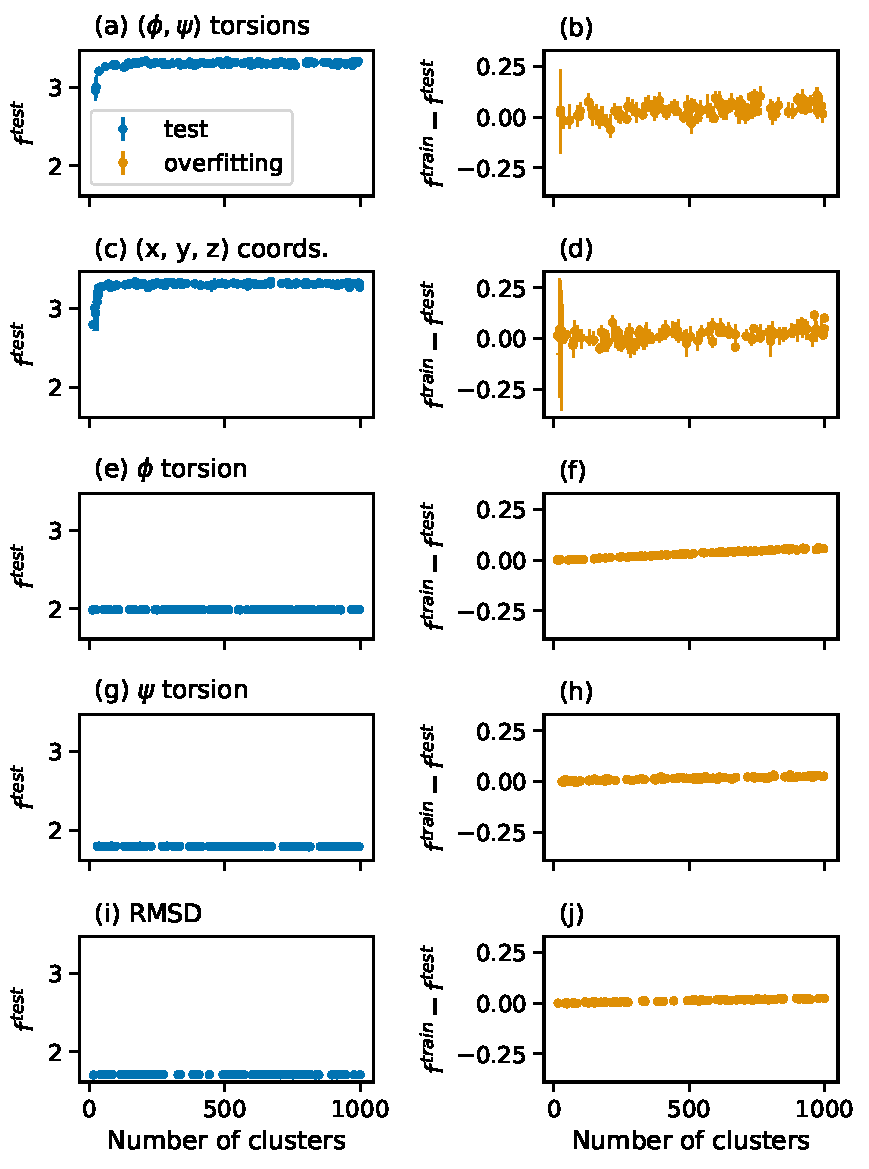
\includegraphics[height=0.8\textheight]{chapters/msm_optimization/figures/ala1_train_test_results.pdf}
    \label{fig:ala1_train_test}
\end{figure}



\subsubsection{Hyperparameter trial data set}

Alanine dipeptide undergoes three relaxation processes which are resolvable with the lag time of $\tau=\SI{9}{\pico\second}$ used here, with implied timescales of approximately $\SI{1300}{\pico\second}$, $\SI{66}{\pico\second}$ and $\SI{30}{\pico\second}$. These values were estimated using a Markov state model using the $(\phi, \psi)$  torsion feature and $n=100$ microstates and are inline with other studies using this data e.g., \cite{varolgunesInterpretableEmbeddingsMolecular2020, mardtVAMPnetsDeepLearning2018}.  As the eigenvalue associate with each relaxation timescale can be at most \num{1}, there is an upper-bound on the VAMP-2 score of \num{4} (this includes the eigenvalue of exactly one corresponding to the stationary distribution, see chapter \ref{chap:theory} section \ref{sec:theory_choice_hyp}). The maximum values of the VAMP-2 score ($\simeq 3.25$) are below this bound and similar to the values estimated in reference \cite{mardtVAMPnetsDeepLearning2018}.  The total length of the MD data set used to create the hyperparameter trial data set is \SI{750}{\nano\second}, which is over \num{500} times as long as this longest relaxation timescale. The implied timescales and volume of simulation data imply that the simulations are well converged. 

The response of a Markov state model to the type of protein feature ($\chi$) and number of cluster centers ($n$) was measured by the cross-validated VAMP-2 score ($f$) using the first five eigenvalues of the transition matrix. The hyperparameter trial data set consisted of 500 observations of $f$ and $(\chi, n)$ and is shown in figure \ref{fig:ala1_train_test}. The test response ($f^{\mathrm{test}} = f\left(\chi, n; \mathbf{X}^{\mathrm{test}}\right)$, blue points) and the difference between train and test response, ($\Delta f = f^{\mathrm{train}} - f^{\mathrm{test}}$, orange) are both shown as functions of $n$. The features are ordered according to the  mean of the test response. As expected from previous work \cite{bolhuis2000reaction} the  $(\phi, \psi)$ feature has the highest average response but figure \ref{fig:ala1_train_test} also shows that the heavy atom $(x,y,z)$ coordinates feature performs just as well. 

The difference between the train and test response, the \emph{over-fitting}, reflects the consistency between the eigenvectors estimated on the training data and those implied from the time-lagged covariance and overlap matrices ($C$ and $\Pi$  in \ref{eqn:tran_def}) estimated  on the test data \cite{mcgibbonVariationalCrossvalidationSlow2015}. So a small $\Delta f$ implies that the picture of the relaxation processes are represented equally well, with the given hyperparameters, in both the training and test data (even if they're both inaccurate). This is likely due to the large volume of data used to train the MSMs. 



\subsubsection{Gaussian process regression}

\begin{figure}
    \centering
    \caption[Response surface of alanine dipeptide]{\textsc{Response surface of alanine dipeptide}. The response is shown as a function of the feature, $\chi$ (panels (a) - (e)) and number of clusters, $n$ (horizontal axis). The features are ordered according to their average response. A Mat\'{e}rn 5-2 kernel and logarithmic warping of the predictor $n$  was used. The blue line is the mean of the surface, the blue shaded bands represent the uncertainty ($\pm2\sigma$ excluding the noise term $\sigma_{n}$), and the black crosses are the observed values (the cross validated mean of VAMP-2).}
    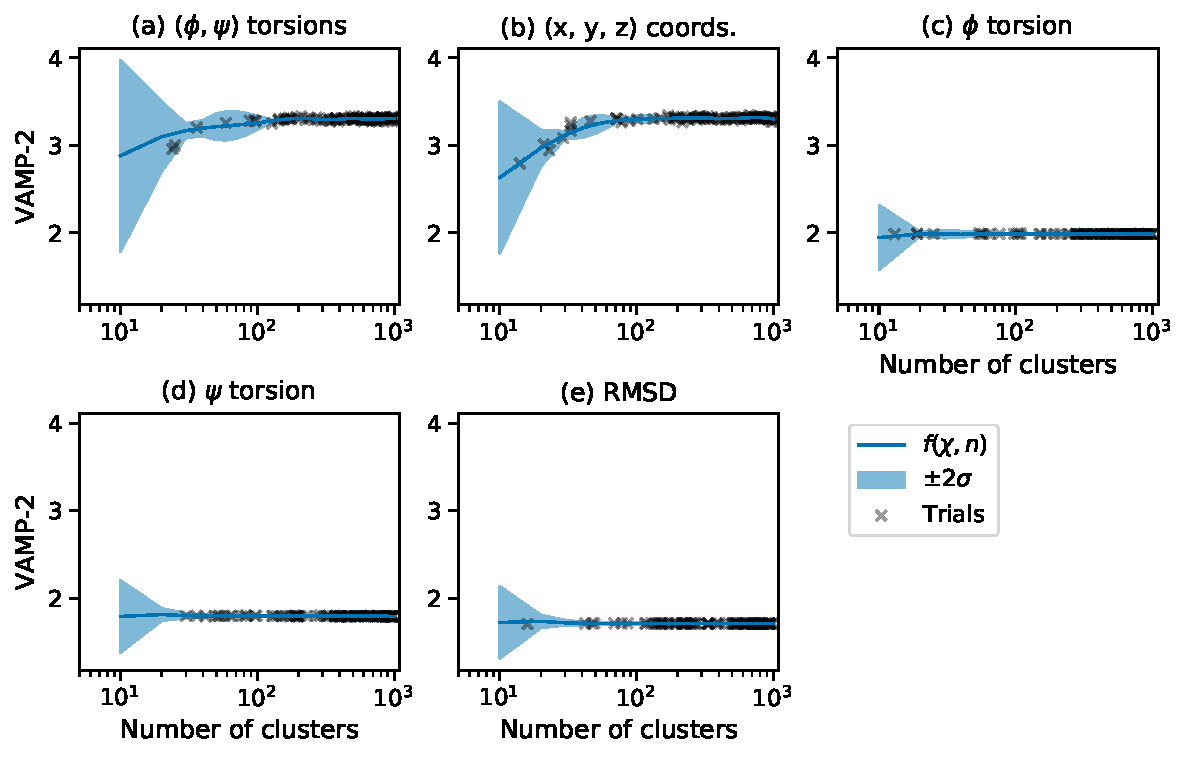
\includegraphics[width=0.8\textwidth]{chapters/msm_optimization/figures/ala1_response_surface.pdf}
    \label{fig:ala1_response}
\end{figure}

The response surface (figure \ref{fig:ala1_response}) was modelled as a Gaussian process with $\chi$ and $n$ as predictors. A Mat\'{e}rn 5-2 kernel and logarithmic input warping of $n$ were chosen using a combination of the MSLL and SMSE model selection criteria. The SMSE and MSLL of the response surface was \num{0.0007} and  \num{-4.2369} respectively, see table \ref{tab:ala2_fit_results} for the selection metrics of all the models. The choice of logarithmic warping of $n$ is unsurprising given that the response for the $(\phi, \psi)$ and $(x,y,z)$ features (panels (a) and (c) in figure \ref{fig:ala1_train_test}) is a clearly non-stationary process: the covariance of the response with respect to changes in $n$ is much lower for $n\leq 100$ than for $n\geq 100$ where the response reaches a plateau. The log transformation smooths the response with respect to $n$ and makes the assumption of a stationarity more plausible.  

The categorical inputs (the protein feature, $\chi$) posed no problems for GP model, the response surface fits the observed data well across each feature, both in terms of the mean response and its uncertainty. 

\subsubsection{Response surface features}

\begin{figure}
    \centering
    \caption[Discretization error of the second right eigenfunction of alanine dipeptide as a function of the number of microstates]{\textsc{Discretization error of the second right eigenfunction of alanine dipeptide as a function of the number of microstates}. The feature used is the $\phi$ backbone torsion. Panel (a) shows the free energy along this feature. Panels (b), (c) and (d) show the normalized MSM right eigenfunction (blue line) estimated $n=2, 10$ and $50$ cluster centers respectively. This is compared with the same eigenfunction estimated with $n=500$ cluster centers (black line). The red shaded area represents the difference between the two eigenfunctions. The discretization error, labelled $\delta$ is the integral of the red area. The $VAMP-2$ score is also labelled for comparison.}
    \label{fig:ala1_evcompare}
    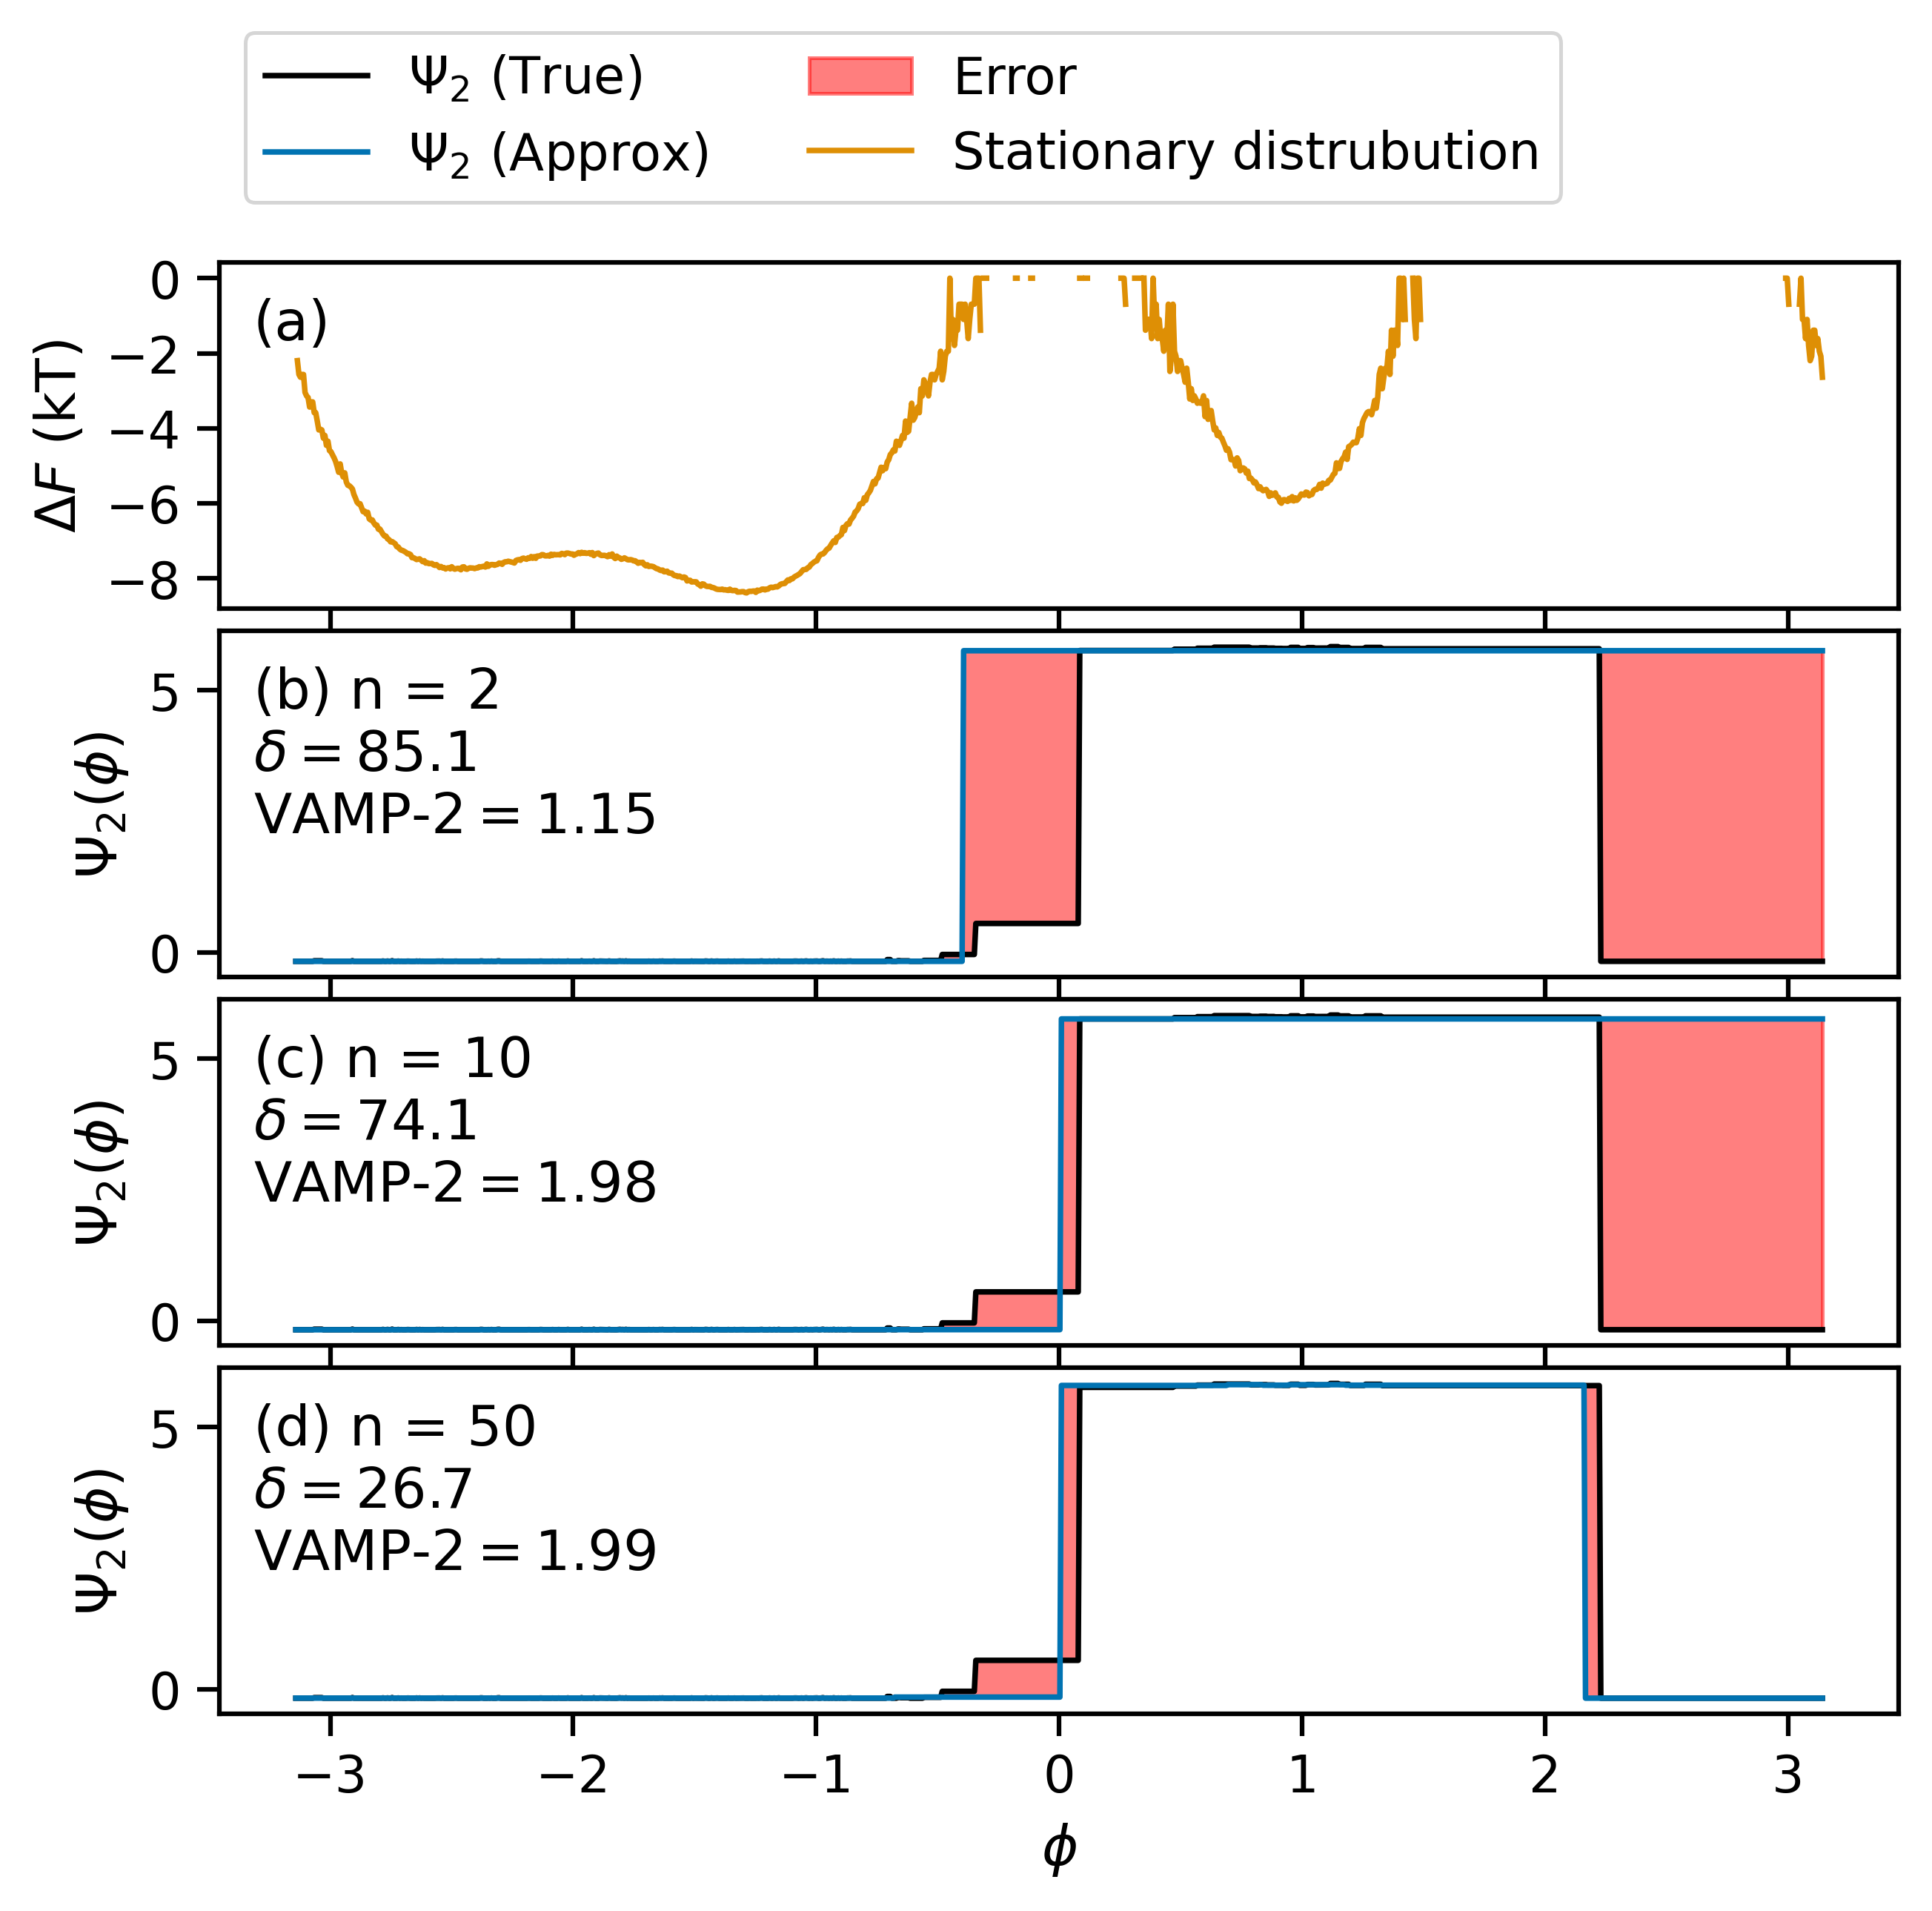
\includegraphics[width=0.8\textwidth]{chapters/msm_optimization/figures/ala1_ev_n_compare.png}
\end{figure}

The three aims of this chapter are to demonstrate the ability of GPs to model the response surface of an MSM, use this response surface to understand the sensitivity of MSMs to their hyperparameters, and optimise the response surface with respect to its hyperparameters. The previous section showed the success of the GP model for modelling the alanine dipeptide response surface.  Before moving on to the next two aims, there are a number of features of the response surface that are worth discussing.  It should be noted that although this simulation data has been used in a variety of molecular kinetics studies \cite{wehmeyerTimelaggedAutoencodersDeep2018a, nuskeMarkovStateModels2017b, nuskeCoarsegrainingMolecularSystems2019, wangMachineLearningCoarseGrained2019, liNeuralCanonicalTransformation2020, varolgunesInterpretableEmbeddingsMolecular2020, nuskeSpectralPropertiesEffective2021, sechiEstimationKoopmanGenerator2021, mardtVAMPnetsDeepLearning2018}, this is the first explicit estimation of an MSM response surface which means only qualitative comparisons can be to other studies. 

First, there is a decrease in response as $n \rightarrow 10$ for the $(\phi, \psi)$ and $(x,y,z)$ coordinate features. Qualitatively this decrease with $n$ is in agreement with previous studies on other systems \cite{wuVariationalApproachLearning2020c,mcgibbonVariationalCrossvalidationSlow2015} and is due to increasing eigenfunction discretization error, $\delta$ \cite{prinzMarkovModelsMolecular2011} as a $n$ decreases. The discretization error measures the difference between the true eigenfunction and the eigenfunction approximated using discrete microstates and is given by \cite{prinzMarkovModelsMolecular2011}:
\begin{equation}\label{eqn:disc_error}
    \delta_{i} \equiv\left\|\Psi_{i}\left(\mathbf{z}\right)-\hat{\Psi}_{i}\left(\mathbf{z}\right)\right\|_{\pi, 2}=\left(\int_{\Omega} d \mathbf{z} \pi(\mathbf{z})(\Psi_{i}(\mathbf{z})-\hat{\Psi}_{i}(\mathbf{z}))^{2}\right)^{1 / 2}
\end{equation}
Here $\mathbf{z}$ are the coordinates of state space (in this case the $\phi$ dihedral angle), $\pi$ is the stationary distribution and the integral runs over all of the state space, $\Omega$. The integrand is the difference between the true normalized eigenfunction $\Psi$ and approximate eigenfunction $\hat{\Psi}$. As the number of microstates decreases, $\hat{\Psi}_{i}$ is not fine-grained enough to capture variations in $\Psi_{i}$, resulting in large values of $\delta_{i}$. In the language of statistical learning theory \cite{friedman2001elements}, a model with errors due to insufficient flexibility in the model definition, in this case too few microstates, is in the high ``bias'' regime of the ``bias-variance'' trade-off. 

In contrast, the response is flat for the $\phi$ and $\psi$ and the RMSD features, which is not expected. This could be because the values of $n$ sampled were not low enough to show discretization error, because of some feature of the simulation data, or due to some error of calculation. In order to understand this, a more detailed investigation of of the relationship between the number of cluster centers, $n$, the eigenvalue discretization error, $\delta$, and the VAMP-2 response was carried out. This is shown for the $\phi$ torsion feature in figure \ref{fig:ala1_evcompare}.  Panel (a) shows the empirical free energy along the $\phi$ torsion in order to provide a point of reference for the remaining panels. The truncation of the free energy around the values of $\phi \simeq 0,\ 2$ radians is due to the low temporal resolution  of the MD trajectories (each frame is separated by \SI{1}{\pico\second}). This truncation is shown in the figures of references \cite{nuskeCoarsegrainingMolecularSystems2019, liNeuralCanonicalTransformation2020, wangMachineLearningCoarseGrained2019, varolgunesInterpretableEmbeddingsMolecular2020, nuskeSpectralPropertiesEffective2021, mardtVAMPnetsDeepLearning2018} which also use this data.  

Panels (b) - (d) show the difference between the `true' (black solid line) and approximate eigenfunctions (blue solid line) for the slowest relaxation process, $\Psi_{2}$. This is the processes which takes the system from the free energy basin on the left-hand side (centered around $\phi\simeq -2$  radians), to the minima on the right hand side  ($\phi \simeq +1$ radians). The `true' eigenfunction was taken as $\Psi_{2}$ estimated with $n=1000$ basis states using the $\phi$ feature (the shape of the eigenvector changed only slightly over the range $[100, 1000]$). Although the true dominant eigenfunction requires both the $\phi$ and $\psi$ torsion angles to be described exactly, for the purposes of seeing the effect of $n$ on the discretization error, this definition suffices. As $n$ increases from $2$ to $10$ to $50$, $\delta$ decreases from $85.1$ to $74.1$ to $26.7$ (this is the sum of the red shaded area) while the VAMP-2 response increases from $1.25$ to $1.98$ to $1.99$. For this feature, and likely for the other one-dimensional features ($\psi$, RMSD), the largest decrease in VAMP-2 occurs below $n=10$ which explains why a drop in VAMP-2 response with decreasing $n$ is not observed. 


Second, the response for all features for $n > 100$ is constant. This due to a number of possible factors. First is the large volume of MD simulation data used to train the MSMs. The discretization error will eventually become negligible for all of the  non-trivial eigenvectors used in the VAMP-2 score as $n$ increases. As already mentioned, this explains the rapid increase in the response for $n<100$. As $n$ increases the statistical uncertainty in the elements of the estimated transition matrix will increase and the model enters the high variance regime of the ``Bias-variance'' trade-off.  However, with the large volume simulation data the number of observations ($750\times(1000-9) = \num{743250}$ pairs of observed transitions) is comparable to the degrees of freedom for a reversible MSM ($\sfrac{1}{2}n(n-1)+n-1=\num{500499}$ for $n=1000$), and so the high-variance regime might be at $n>1000$. Second, the temporal resolution of the trajectories was not high enough to resolve all the slow relaxation processes stipulated in the VAMP-2 score and so increasing $n$ did not increase the accuracy of the eigenvectors.  This is demonstrated in panel (a) of figure \ref{fig:ala1_evcompare} where the truncation in the free energy surface indicates the upper limit of the resolution. 

This flat behaviour is in contrast to other studies \cite{mcgibbonVariationalCrossvalidationSlow2015,wuVariationalApproachLearning2020c,prinzMarkovModelsMolecular2011} where the size of the microstates is important for optimising the MSM. However, with these studies indicator basis function were used whose definition are not dependent on the data. This points to the possibility that for measuring the slow processes, the k-means method which adapts the definition of the state to the data at hand, may not have a practical upper limit on the number of cluster centers (below the pathological limit of the total number of observations). 

The third feature of the response surface is the large uncertainty of response surface for $n \leq 20$ which is a result of the comparatively sparse sampling in this region. This was because all sampling was done without prior logarithmic warping, which would have placed more important on small values of $n$ and increased the density of samples in this region.  
 
\subsubsection{Practical implications}

A Gaussian process regression model can be used to model the VAMP-2 response of a Markov state model to both integer valued hyperparameters (number of microstates) and categorical variables (the protein feature). A fully multiplicative kernel of the type in equation \ref{eqn:kernel_form} can by used to model multiple  hyperparameters, while different kernel functions can be selected by choosing the model with the best combination of standardize log loss and mean square error. Although this is not useful in isolation, this is an important stepping stone to both measuring hyperparameter relevance and optimising MSMs. 

 
\subsection{Hyperparameter relevance}\label{subsubsec:ala_relevance}

\begin{figure}
    \centering
    \caption[Relevance of the hyperparameters of alanine dipeptide]{\textsc{Relevance of the hyperparameters of alanine dipeptide}. The distribution of the parameters of the response surface (shown in figure \ref{fig:ala1_response}) were estimated using MCMC. The relevance of the features (levels of $\chi$) are shown in blue, labelled `Feature'. The relevance of the log-transformed number of cluster centres, $n$ is shown in orange (labelled `Other').}
    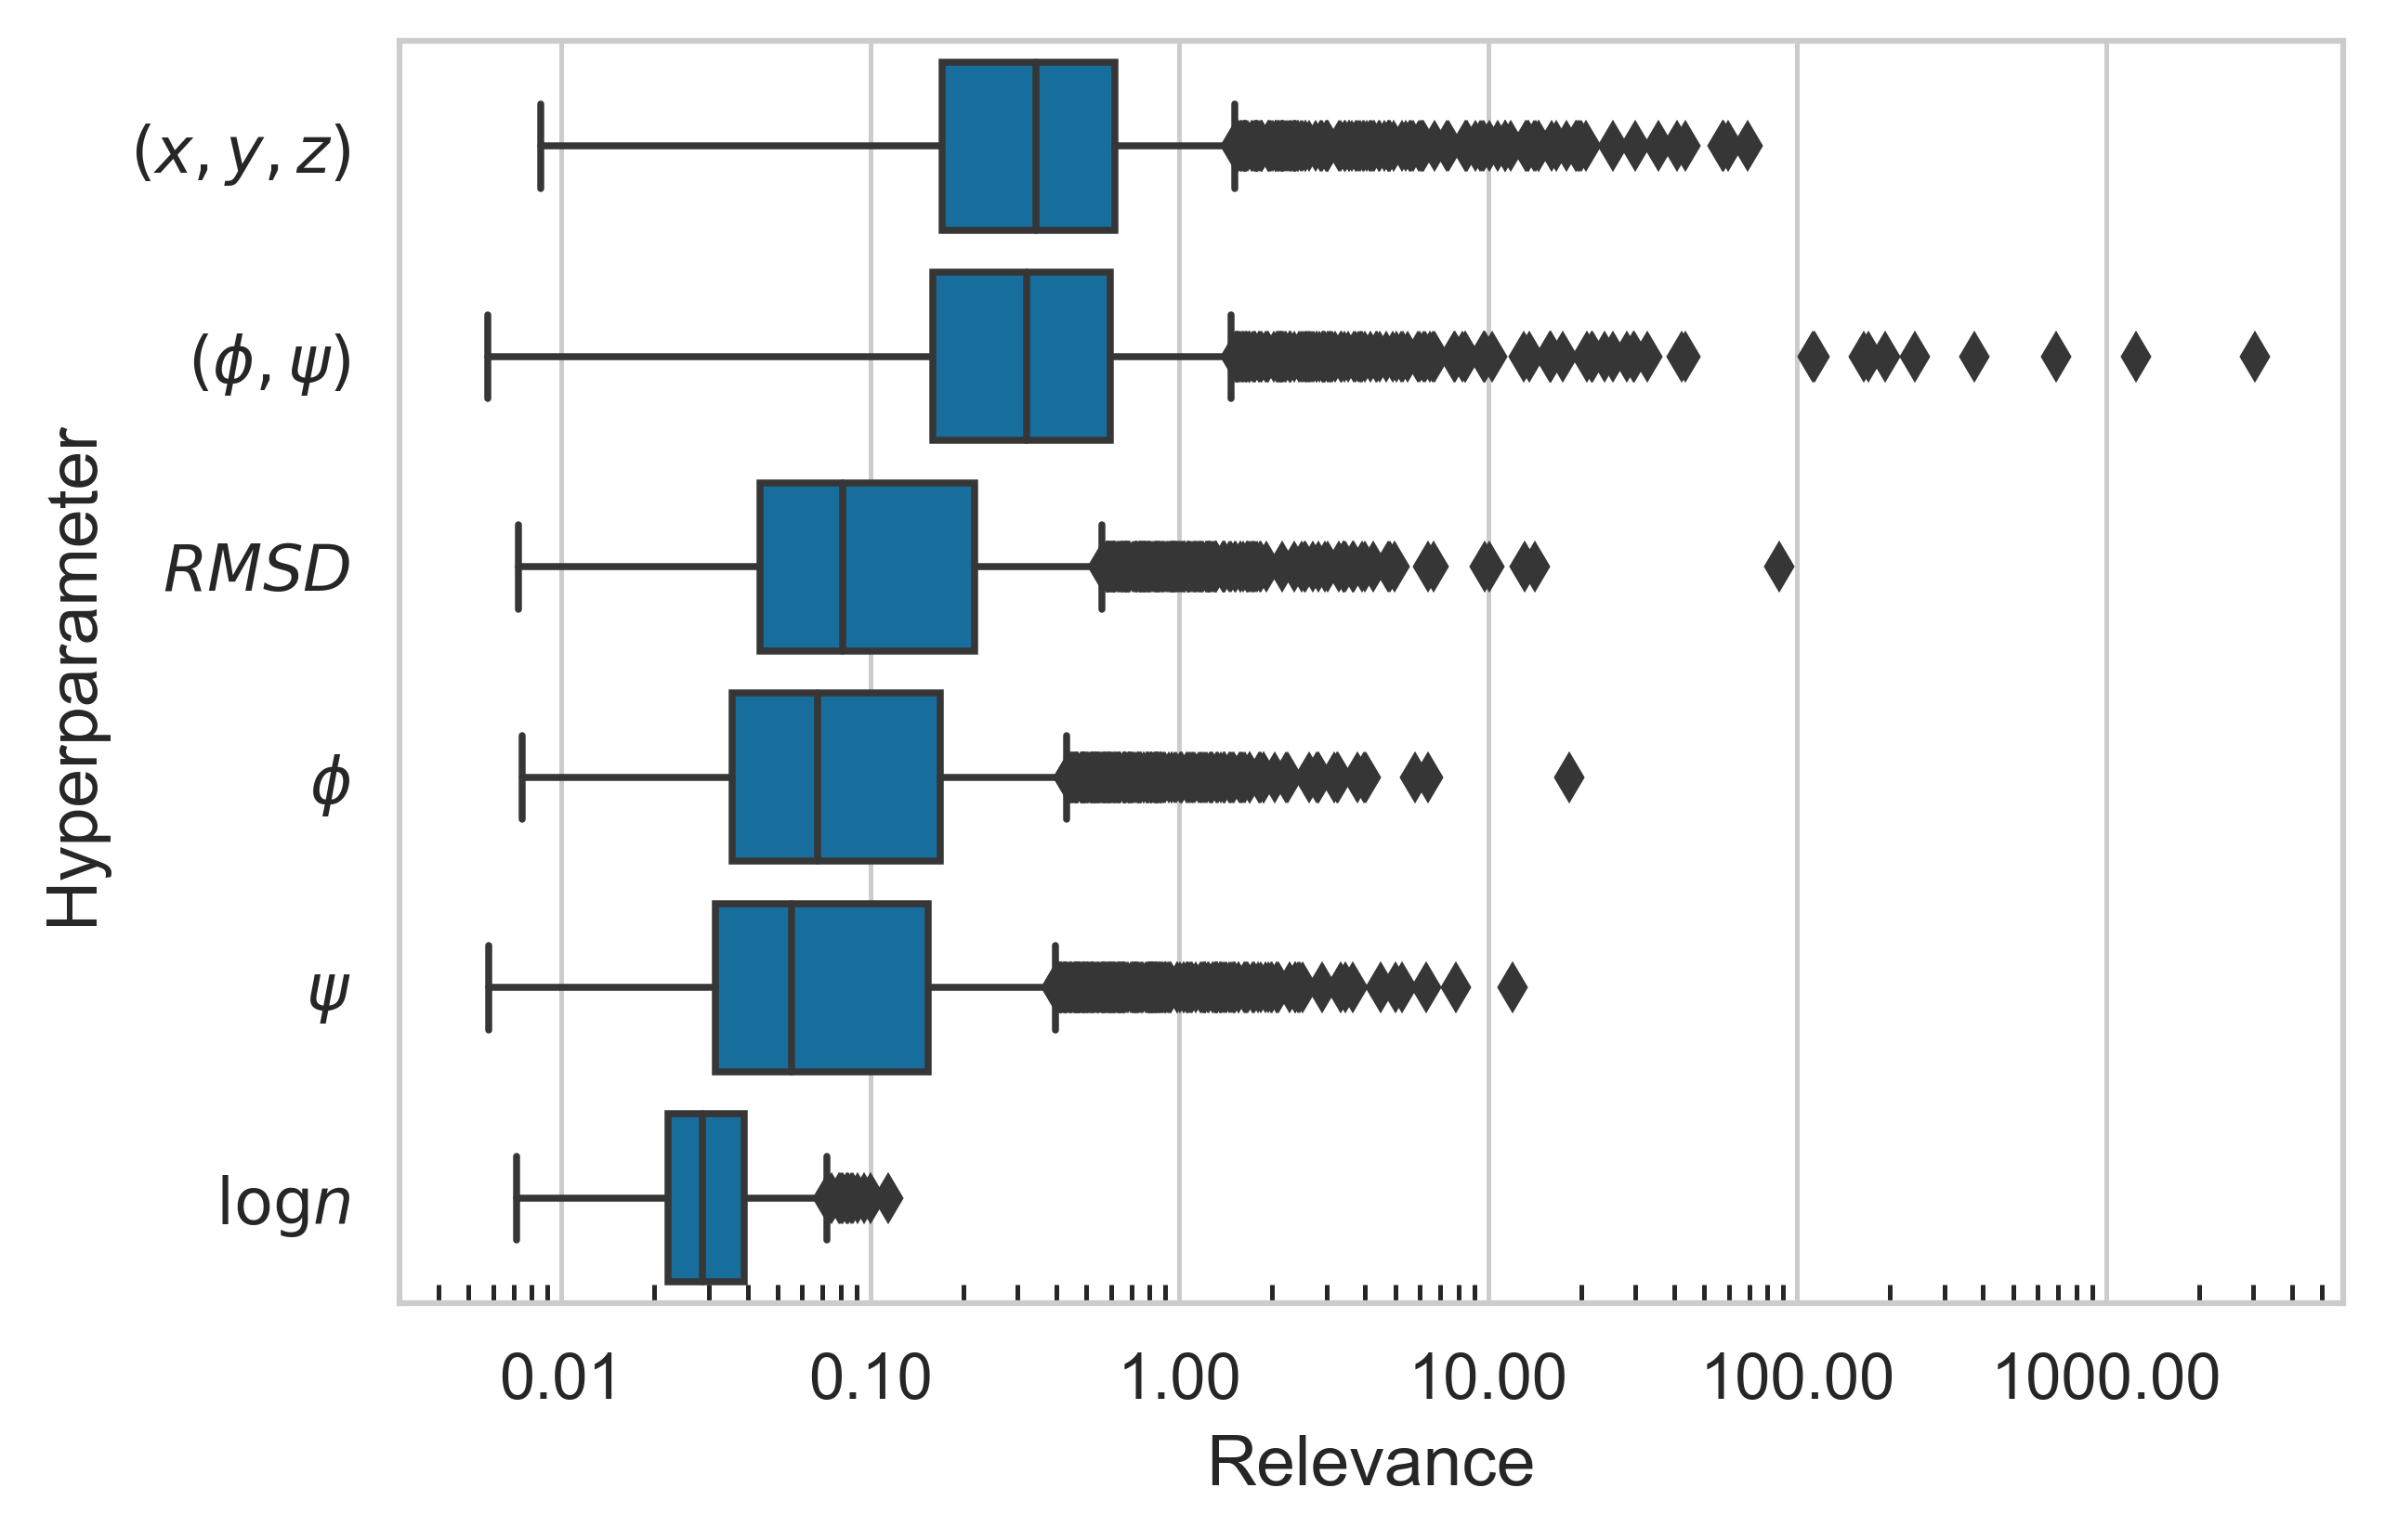
\includegraphics[width=0.8\textwidth]{chapters/msm_optimization/figures/ala1_relevance.png}
    \label{fig:ala1_relevance}
\end{figure}

\begin{table}
    \centering
    \caption[Posterior distribution of GP hyperparameters]{\textsc{Posterior distribution of GP hyperparameters}. Median and $\SI{95}{\percent}$ credible intervals for the kernel hyperparameters of the alanine dipeptide response surface estimated using MCMC. The length-scale parameters in \ref{eqn:kernel_form} are re-written here as relevances.}
    \begin{tabular}{lrr}
    \toprule
                          Hyper-parameter &    Median & $\SI{95}{\percent}$ C.I. \\
    \midrule
     $R_{(\phi, \psi)\ \mathrm{torsion}}$ &  0.321 & 0.020-4.456 \\
        $R_{(x, y, z)\ \mathrm{coords.}}$ &  0.344 & 0.024-5.572 \\
             $R_{\phi\ \mathrm{torsion}}$ &  0.068 & 0.015-1.176 \\
             $R_{\psi\ \mathrm{torsion}}$ &  0.056 & 0.013-1.327 \\
                               $R_{RMSD}$ &  0.081 & 0.016-1.406 \\
                          $R_{\log{(n)}}$ &  0.029 & 0.013-0.063 \\
                                   $\eta$ &  2.518 & 1.141-5.530 \\
                               $\sigma_n$ &  0.006 & 0.006-0.007 \\
    \bottomrule
    \end{tabular}
    \label{tab:ala1_rel_post}
\end{table}


The relevance of continuous hyperparameters such as the number microstates $n$ considered here,  determines how sensitive the model response is to changes in hyperparameters. The more relevant a hyperparameter, the  greater the change in model response is to a change its value.  The  relevance of the number of microstates is $0.029\ [\numrange[range-phrase=\text{--}]{0.013}{0.064}]$ (table \ref{tab:ala1_rel_post} and figure \ref{fig:ala1_relevance}). Such a low value indicates that the number of microstates only has a negligible effect on the VAMP-2 response of the MSM. This is also evident from looking at the response surface itself, figure  \ref{fig:ala1_response} which shows the response flat with respect to changes in $n$. The practical implication is that it is not necessary to optimize the number of microstates in an MSM when using k-means clustering (the method used to create the microstates for the models fit here). However, for very small values, the value of $n$ does determine the VAMP-2 score, as was discussed in the previous section. This means that the assumption of stationarity doesn't hold as correlation in the response for low values of $n$ is different to that for large values of $n$. 

% the MSM hyperparameters were calculated from the estimated response surface, using the method described in section \ref{sub:msm_meth_rel}. The results summarised in box plots in figure \ref{fig:ala1_relevance}, and  are also tabulated, along with other GP parameters, in table \ref{tab:ala1_rel_post}. 
% The posterior distributions of the six relevance parameters of the response surface are summarised in box plots in figure \ref{fig:ala1_relevance}, and  the median and $\SI{95}{\percent}$ credible intervals  are tabulated in table \ref{tab:ala1_rel_post}. The interpretation of the relevances of $\chi$ will be different to that of $n$ however. 

Previous work \cite{bergstrajamesbergstraRandomSearchHyperParameter2012} calculated the relevance of continuous hyperparameters only.  This work extends the idea by considering categorical hyperparameters, namely the protein feature $\chi$. The relevance of $\chi$ determines the amount of information sharing between the parts of the response surface with different values of $\chi$. In order to understand this, it will be useful to contrast it with  the relevance of a continuous or integer-valued hyperparameters.  The relevance of $n$ determines the covariance of the response to changes in $n$ \emph{within the same feature}. This can be seen from the equation \ref{eqn:kernel_form} and making use of the fact that all stationary kernel functions, $k(x, x^{\prime})=1$ for $x-x^{\prime}=0$:
\begin{equation*}
\begin{split}
    k^{tot}(\mathbf{x}, \mathbf{x}^{\prime})& = k\left((1, 0, 0, 0, 0, n), (1, 0, 0, 0, 0, n^{\prime})\right) \\
    & = \eta^{2}\cdot 1 \cdot 1\cdot 1 \cdot 1\cdot 1 \cdot k_{M}(n, n^{\prime}; R_{n}) \\
    & = \eta^{2}\cdot k(n, n^{\prime})
\end{split}
\end{equation*}
Here the kernel functions have been re-written with the relevance, $R$, instead of the length-scale $l$ as a hyperparameter. The median relevance of $\log{(n)}$ is equal to $\num{0.029}$ which implies that for change $n=10$ and $n=1000$ (a change of $1$ on the normalized scale) the covariance will be $\eta^{2}k_{M-52}(0,1; 0.029) \simeq 0.99\eta^{2}$. In other words, the response will be independent of the $n$ as already noted. 

The relevance of the different features determines the amount of information sharing between different features \cite{duvenaud2011additive}. Between a high relevance feature and all other features, there is little information sharing; between low relevance features there is a large amount of information sharing. To see this, consider the covariance between points at $n$ and $n^{\prime}$ on two different features, $\chi_1$ and $\chi_2$: 
\begin{equation*}
\begin{split}
    k^{tot}(\mathbf{x}, \mathbf{x}^{\prime})& = k\left((1, 0, 0, 0, 0, n), (0, 1, 0, 0, 0, n')\right) \\
    & = \eta^{2}\cdot k_{M}\left(1, 0; R_{\chi_1}\right) \cdot k_{M}\left(0, 1; R_{\chi_2}\right) \cdot 1 \cdot 1\cdot 1 \cdot k_{M}(n, n^{\prime}; R_{n}) \\
    &=  \eta^{2}\cdot k_{1}\cdot k_{2}\cdot k(n, n^{\prime})
\end{split}
\end{equation*}

If either $R_{\chi_1}$ or $R_{\chi_2}$ is large then $k_1 \cdot k_2 \simeq 0$ and there will no correlation between $n$ on feature $\chi_1$ and $n^{\prime}$ on feature $\chi_2$. If both $R_{\chi_1}$ and $R_{\chi_2}$ are small then $k_1 \cdot k_2 \simeq 1$ and covariance between $n$ on feature $\chi_1$ and $n^{\prime}$ on $\chi_2$ will be similar to the covariance between $n$ and $n^{\prime}$ on the same feature.  

The features for alanine dipeptide are all low relevance which is a reflection of the  consistently flat response to changes in $n$ discussed above. Even between  two largest relevance features $(\phi, \psi)$ (relevance = $0.321\ [\numrange[range-phrase=\text{--}]{0.020}{4.456}]$) and $(x,y,z)$ (relevance = $0.344\ [\numrange[range-phrase=\text{--}]{0.024}{5.572}]$) the covariance between $n$ and $n^{\prime}$ on these two features is only altered by  $k_{1}\cdot k_{2} = 0.91\cdot0.92 \simeq 0.83$. 

\subsubsection{Practical implications}

Using an estimated response surface, the relevance of hyperparameters of an MSM can be estimated. Time should be spent optimising high relevance continuous or integer-valued hyperparameters as small changes in their value imply large changes in model response. High relevance hyperparameters should be chosen for sensitivity tests, which test the robustness of scientific conclusions to modelling choices (not just model outcomes). For  categorical hyperparameters such as the protein feature, $\chi$, the story is subtly different.  A group of low relevance values of a categorical hyperparameter can all be treated similarly with respect to the other hyperparameters. With respect to work here - the optimum value of $n$ is then similar for all values of protein feature.


\subsection{Optimization}\label{sec:ala_opt}

\begin{figure}[p]
    \centering
    \caption[Bayesian optimisation]{\textsc{Bayesian optimisation}. Each column shows the response surface at three sequential points in the Bayesian optimisation procedure and each row corresponds to a different feature. The vertical axis is the MSM response, and the horizontal axis the number of microstates on a logarithmic scale. The blue line and shaded area show the response surface (mean and uncertainty respectively) estimated using the hyperparameter trial data set, shown as small black crosses. The white star shows the incumbent and the black dashed line shows the expected improvement (right hand scale - note different vertical scales for each row). The white cross shows the candidate hyperparameter, i.e., the maximum of the acquisition function. The large black cross show the actual value of the hyperparameter trial that was suggested in the previous column.}
    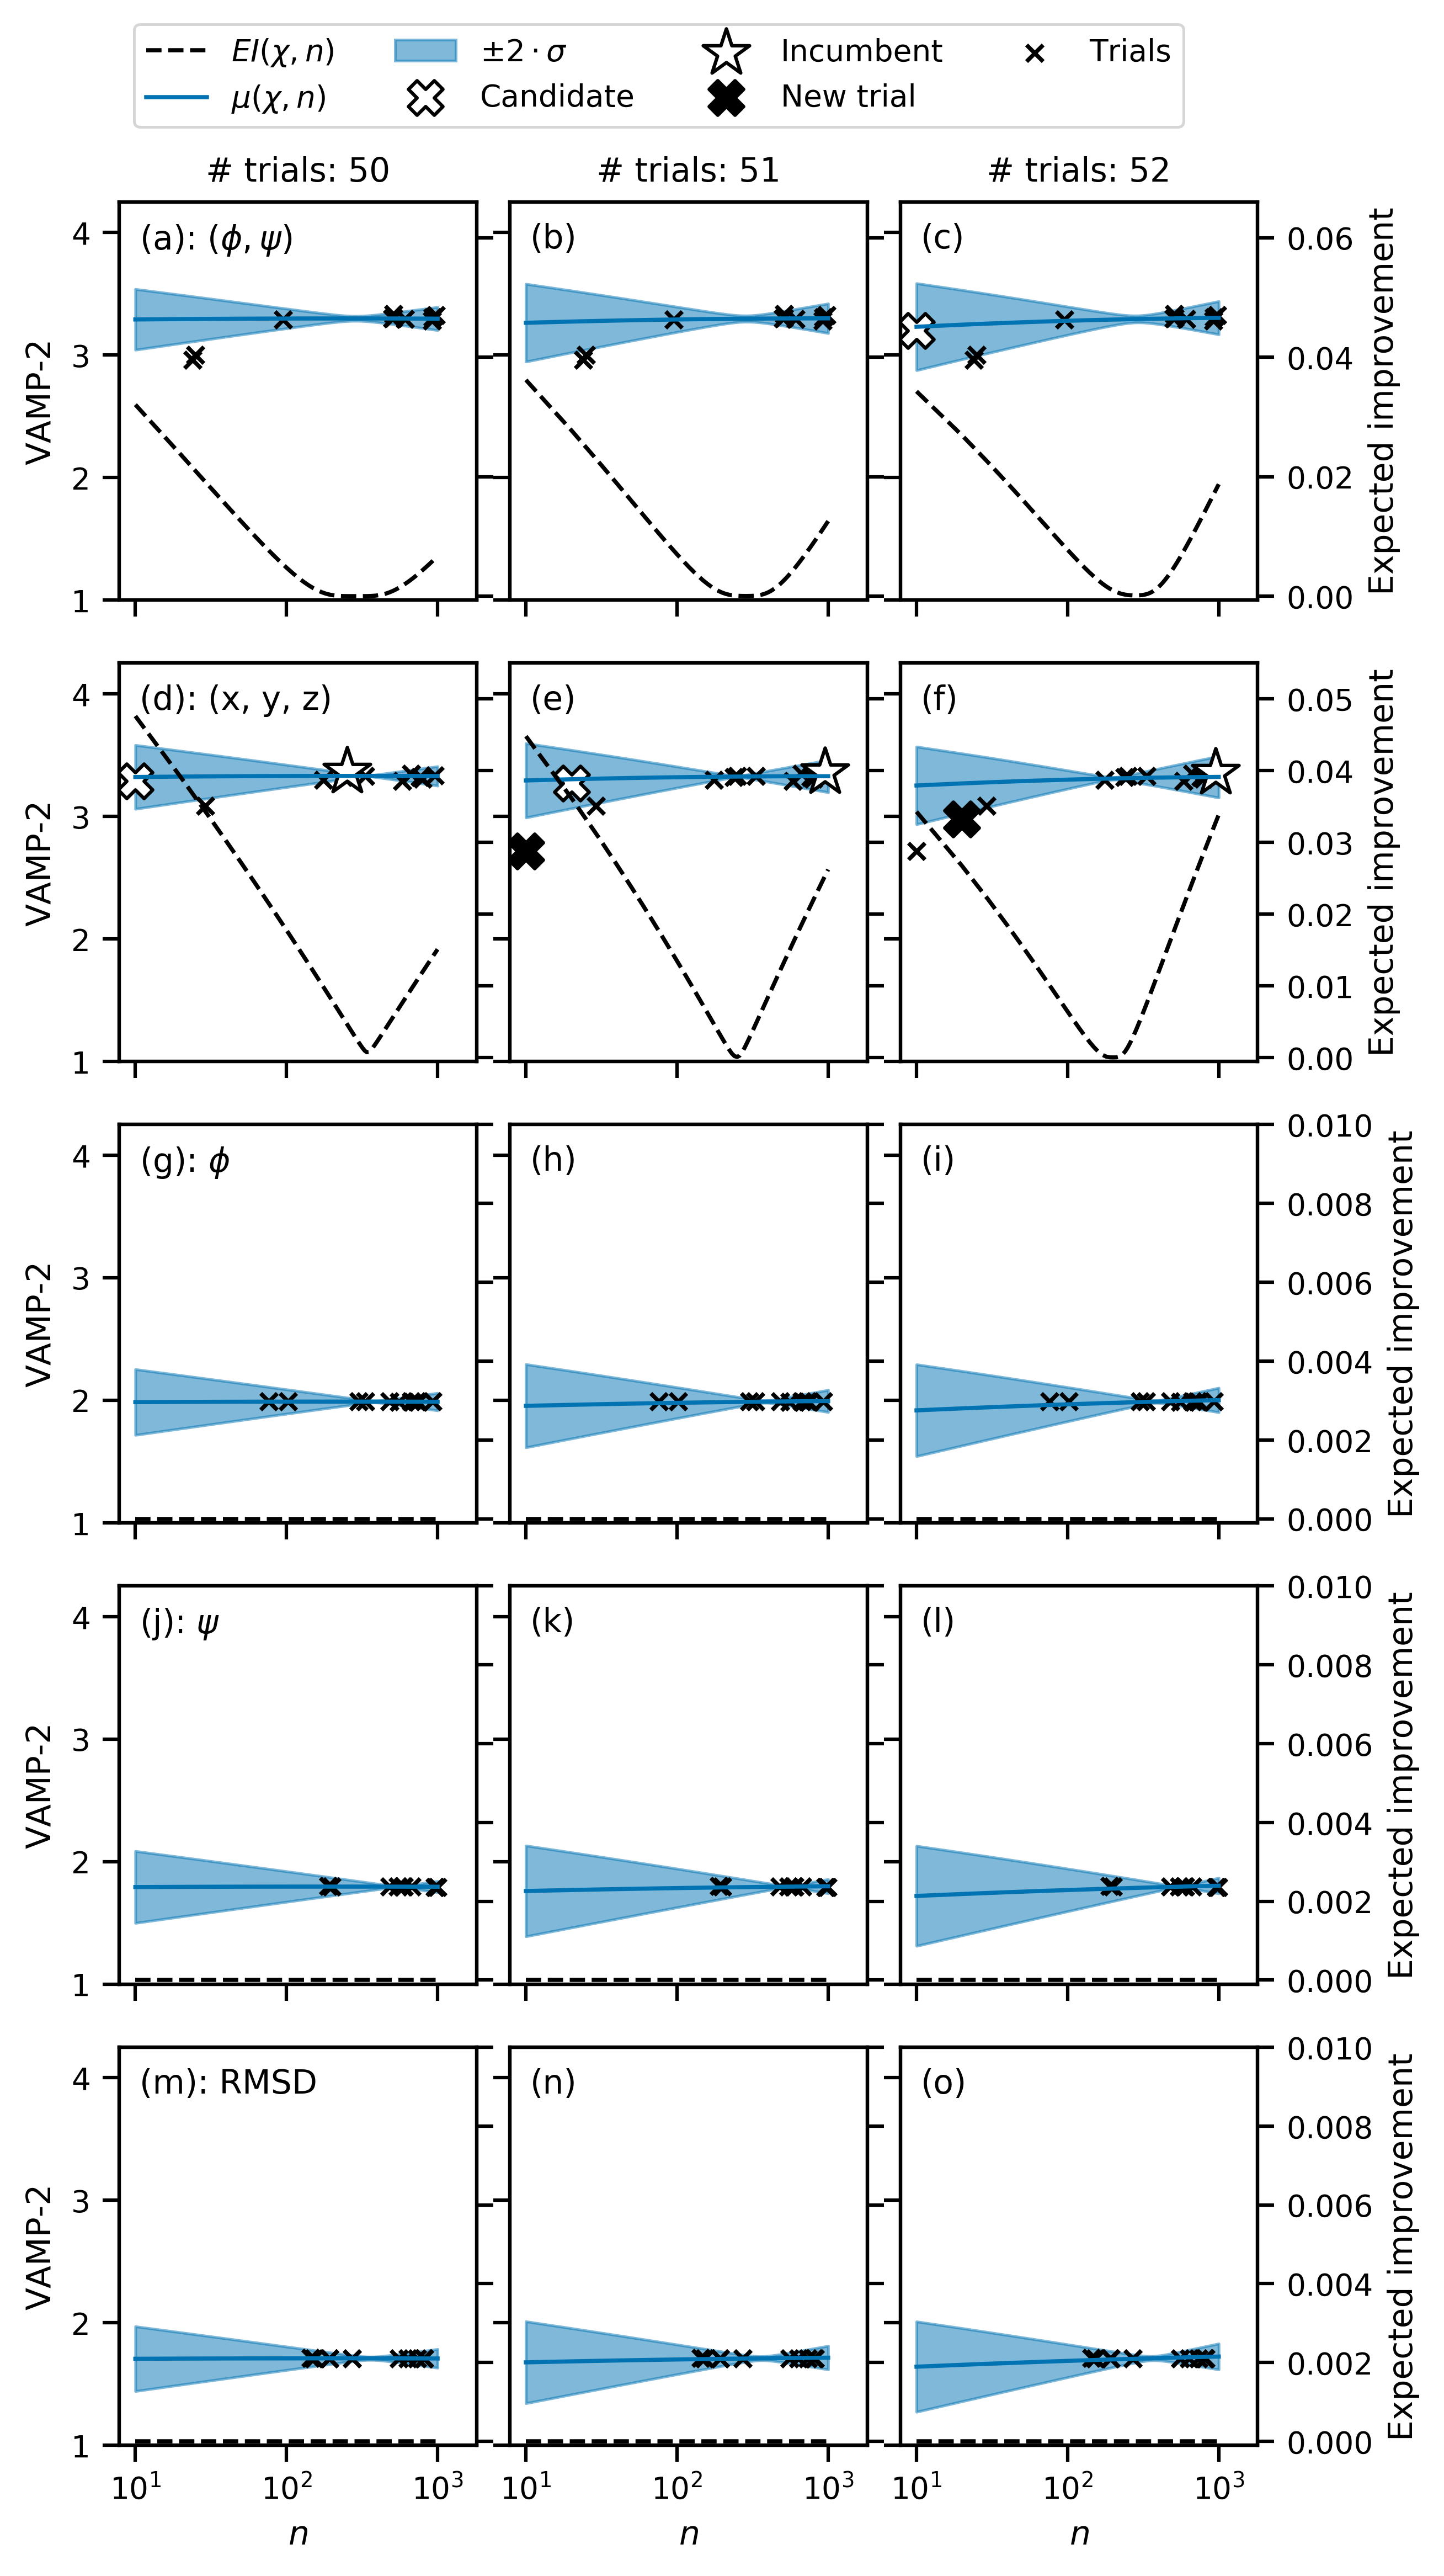
\includegraphics[height=0.75\textheight]{chapters/msm_optimization/figures/ala1_opt_explainer.png}
    \label{fig:msm_opt_explainer}
\end{figure}

The maximum of the response surface \emph{at the trial values} gives the optimum hyperparameters incorporating uncertainty and making full use of all the trial information. For alanine dipeptide, the maximum of the response surface, $\mu=\num{3.318}\pm\num{0.004}$, corresponds to using the $(x, y, z)$ coordinates feature with $n=762$ cluster centers. Given its simplicity, visual inspection of the response surface in figure \ref{fig:ala1_response} was deemed sufficient to confirm that no more sampling was necessary to locate the maximum. 

Bayesian optimisation was used to determine whether this maximum could be achieved using a smaller number of trials and to test the code written to perform the optimisation use in chapter \ref{chap:aadh}. The Bayesian optimisation process for three consecutive steps is demonstrated in figure \ref{fig:msm_opt_explainer}. The first column (panels (a), (d), etc.) shows the response surface estimated using the hyperparameter trial data set with $N=50$ trials. The blue line and shaded area in panel (d) are the response surface with $\chi=(x, y, z)$. The white star is the incumbent - the maximum of the response surface, across all features but only evaluated for $\mathbf{x}\in \mathcal{D}_{50}$. The expected improvement is shown as a dashed line and its maximum corresponds to the point on the response surface denoted by the white cross. This value,  $\mathbf{x}_{50} = \left(\chi=(x, y, z), n=10\right)$ is the candidate and is evaluated in the  next step. In the second column (panels (b), (e) etc.) $\mathbf{x}_{50}$ has been evaluated and the result is shown as a filled black cross. Its value is much smaller than expected, although the new response surface adapts poorly to this information - the mean response does not pass through this new point. This process is repeated in the next column (panels (c), (f) etc.). The white cross in panel (e) is evaluated and shown as a black cross in panel (f) (the candidate in panel (e) is not at the maximum of the acquisition function because the maximum  was the same as the previous step).

\begin{figure}[p]
    \centering
    \caption[Bayesian optimisation trajectories of alanine dipeptide]{\textsc{Bayesian optimisation trajectories of alanine dipeptide}. Shown are five different random subsets  (`iterations') of the total hyperparameter trial data, each separately optimised, seeded with $30$ hyperparameter trials or $15$ observations per predictor (panel (a)), and 50 hyperparameter trials or $25$ observations per predictor (panel (b)). The orange values are the trajectories calculated from random sampling, the blue values are the Bayesian optimisation trajectories. The first row (sub-panels (i) - (v)) are the VAMP-2 response, the second row (sub-panels (vi) - (x)) show the accompanying number of cluster centres, and the third row (sub-panels (xi) - (v)) are the  accompanying feature.}\label{fig:ala_opt_traj}
    \subtop[$N_{ \mathrm{seed}}=30$\label{fig:ala_opt_traj_30}]{
        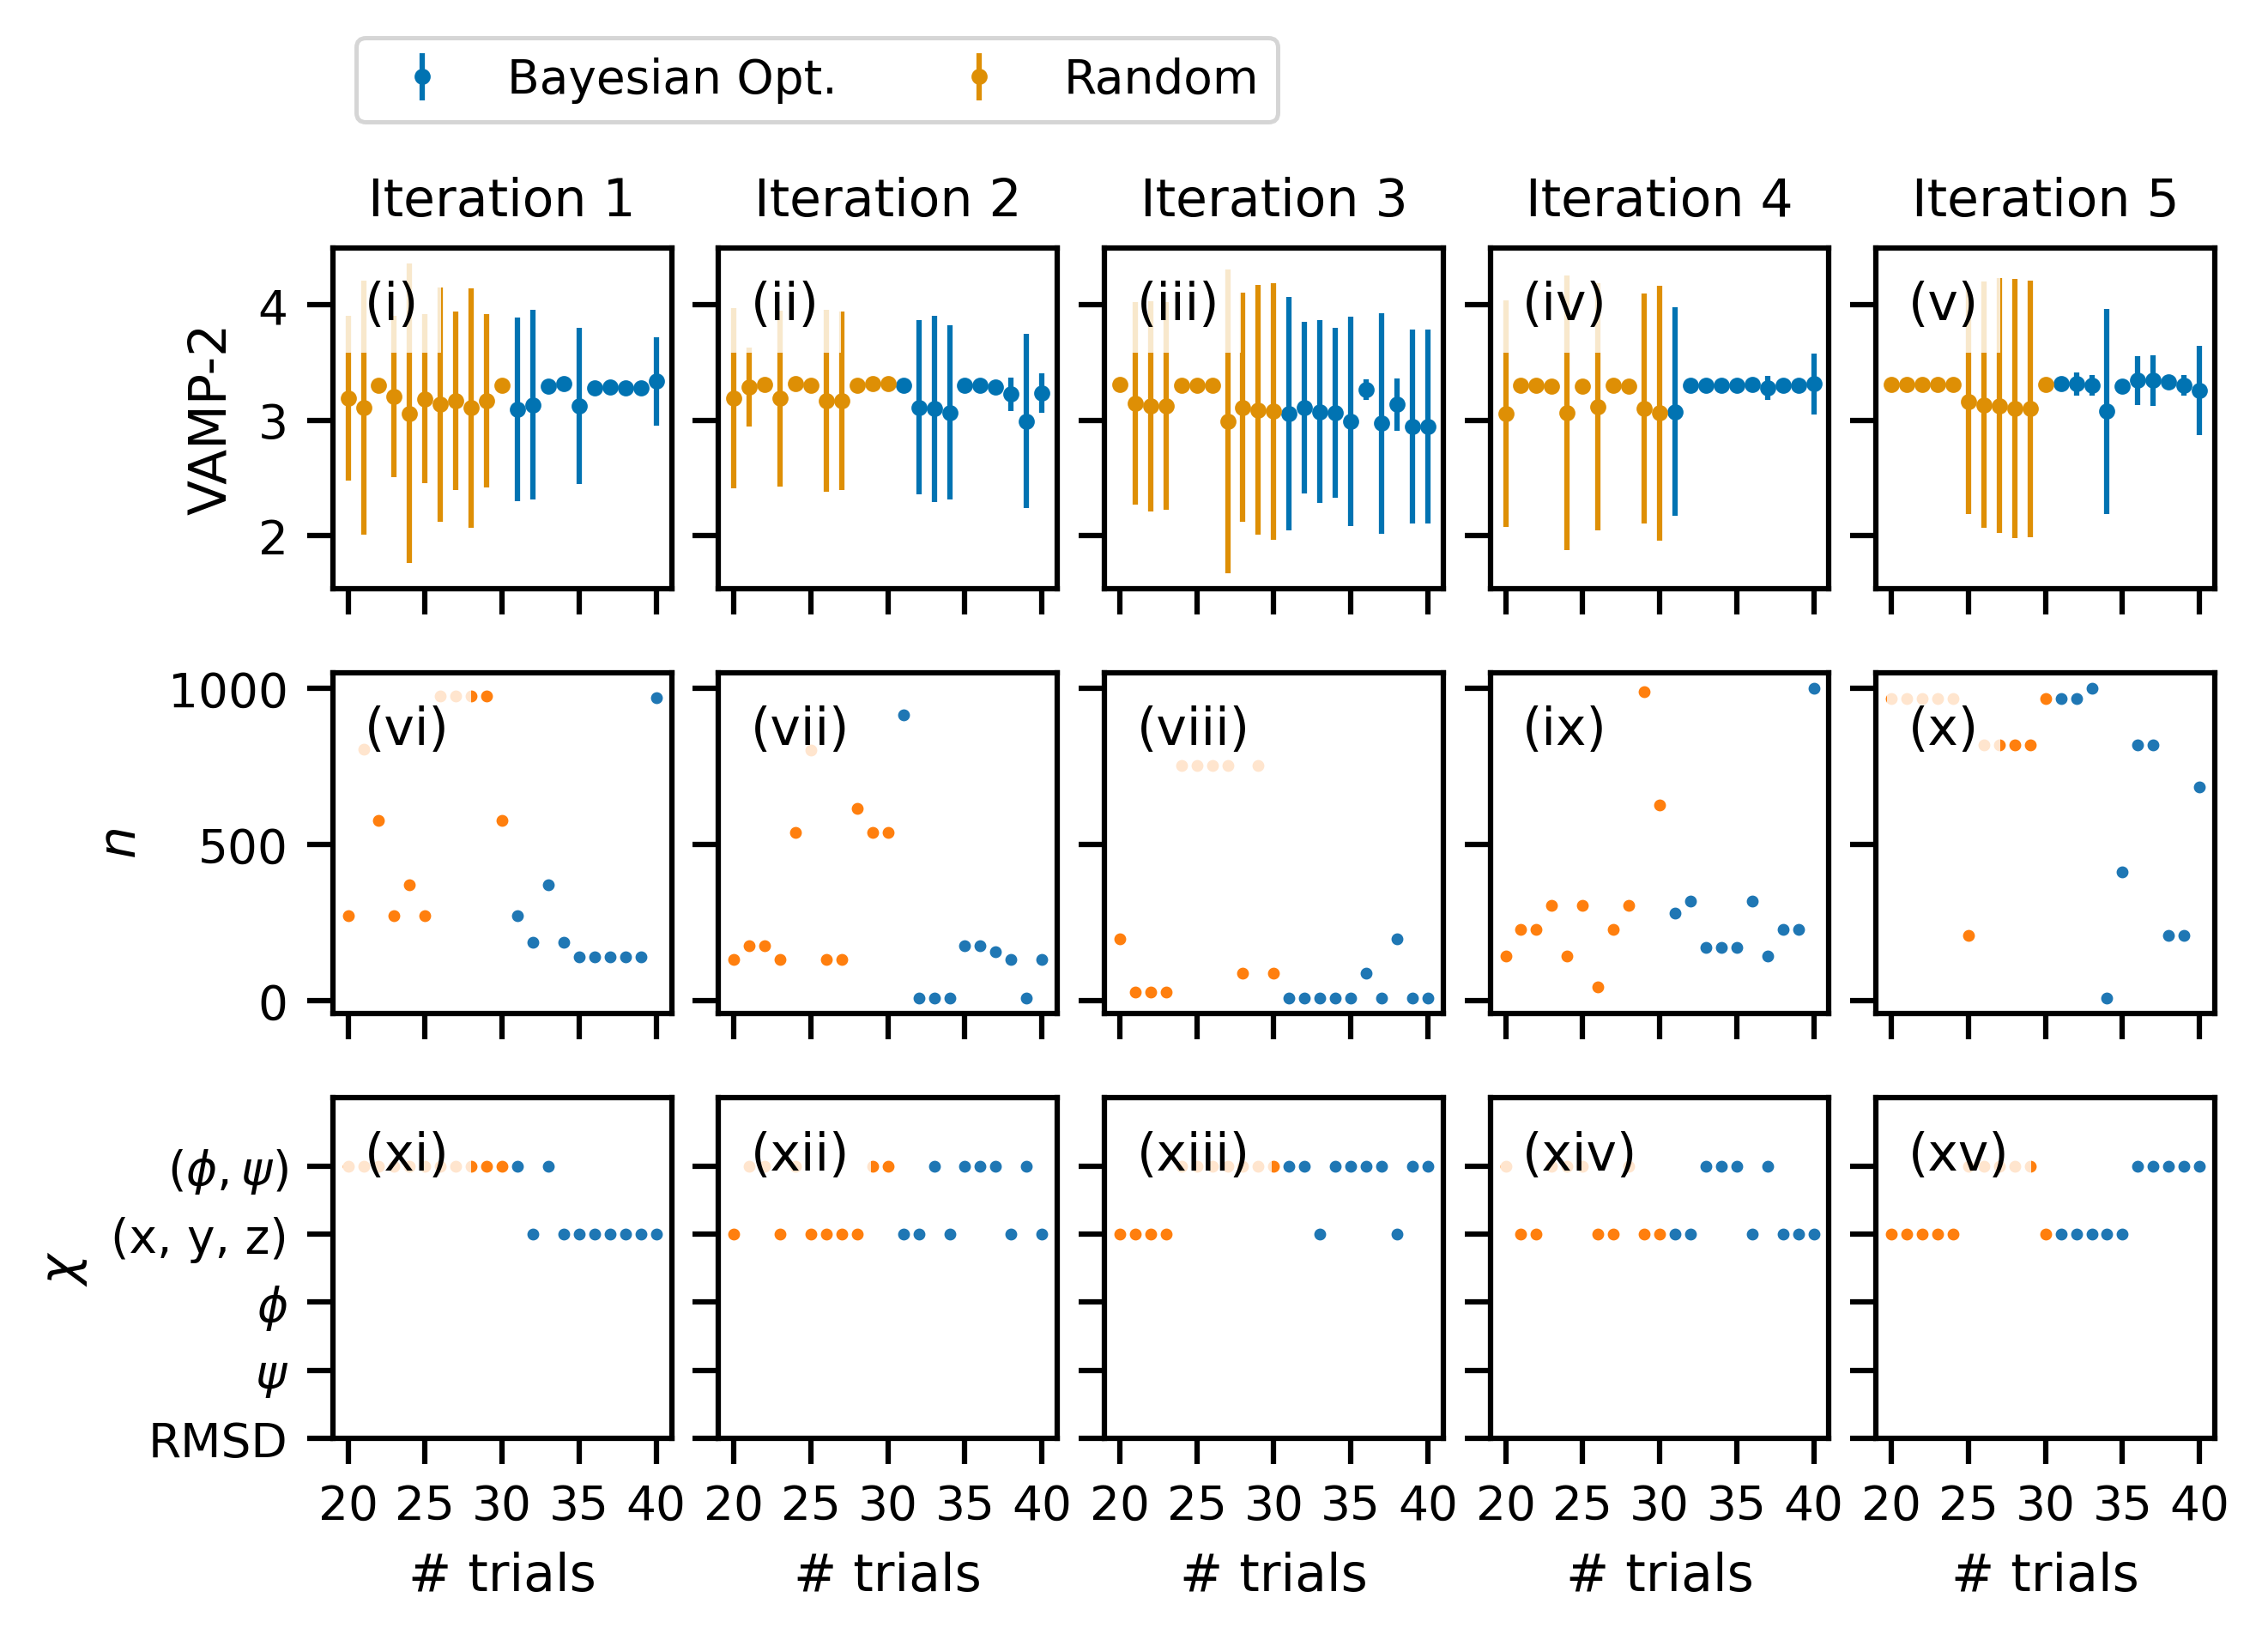
\includegraphics[width=0.7\linewidth]{chapters/msm_optimization/figures/ala1_opt_traj_start_obs_30.png}}
    \subtop[$N_{\mathrm{seed}}=50$ \label{fig:ala_opt_traj_50}]{
        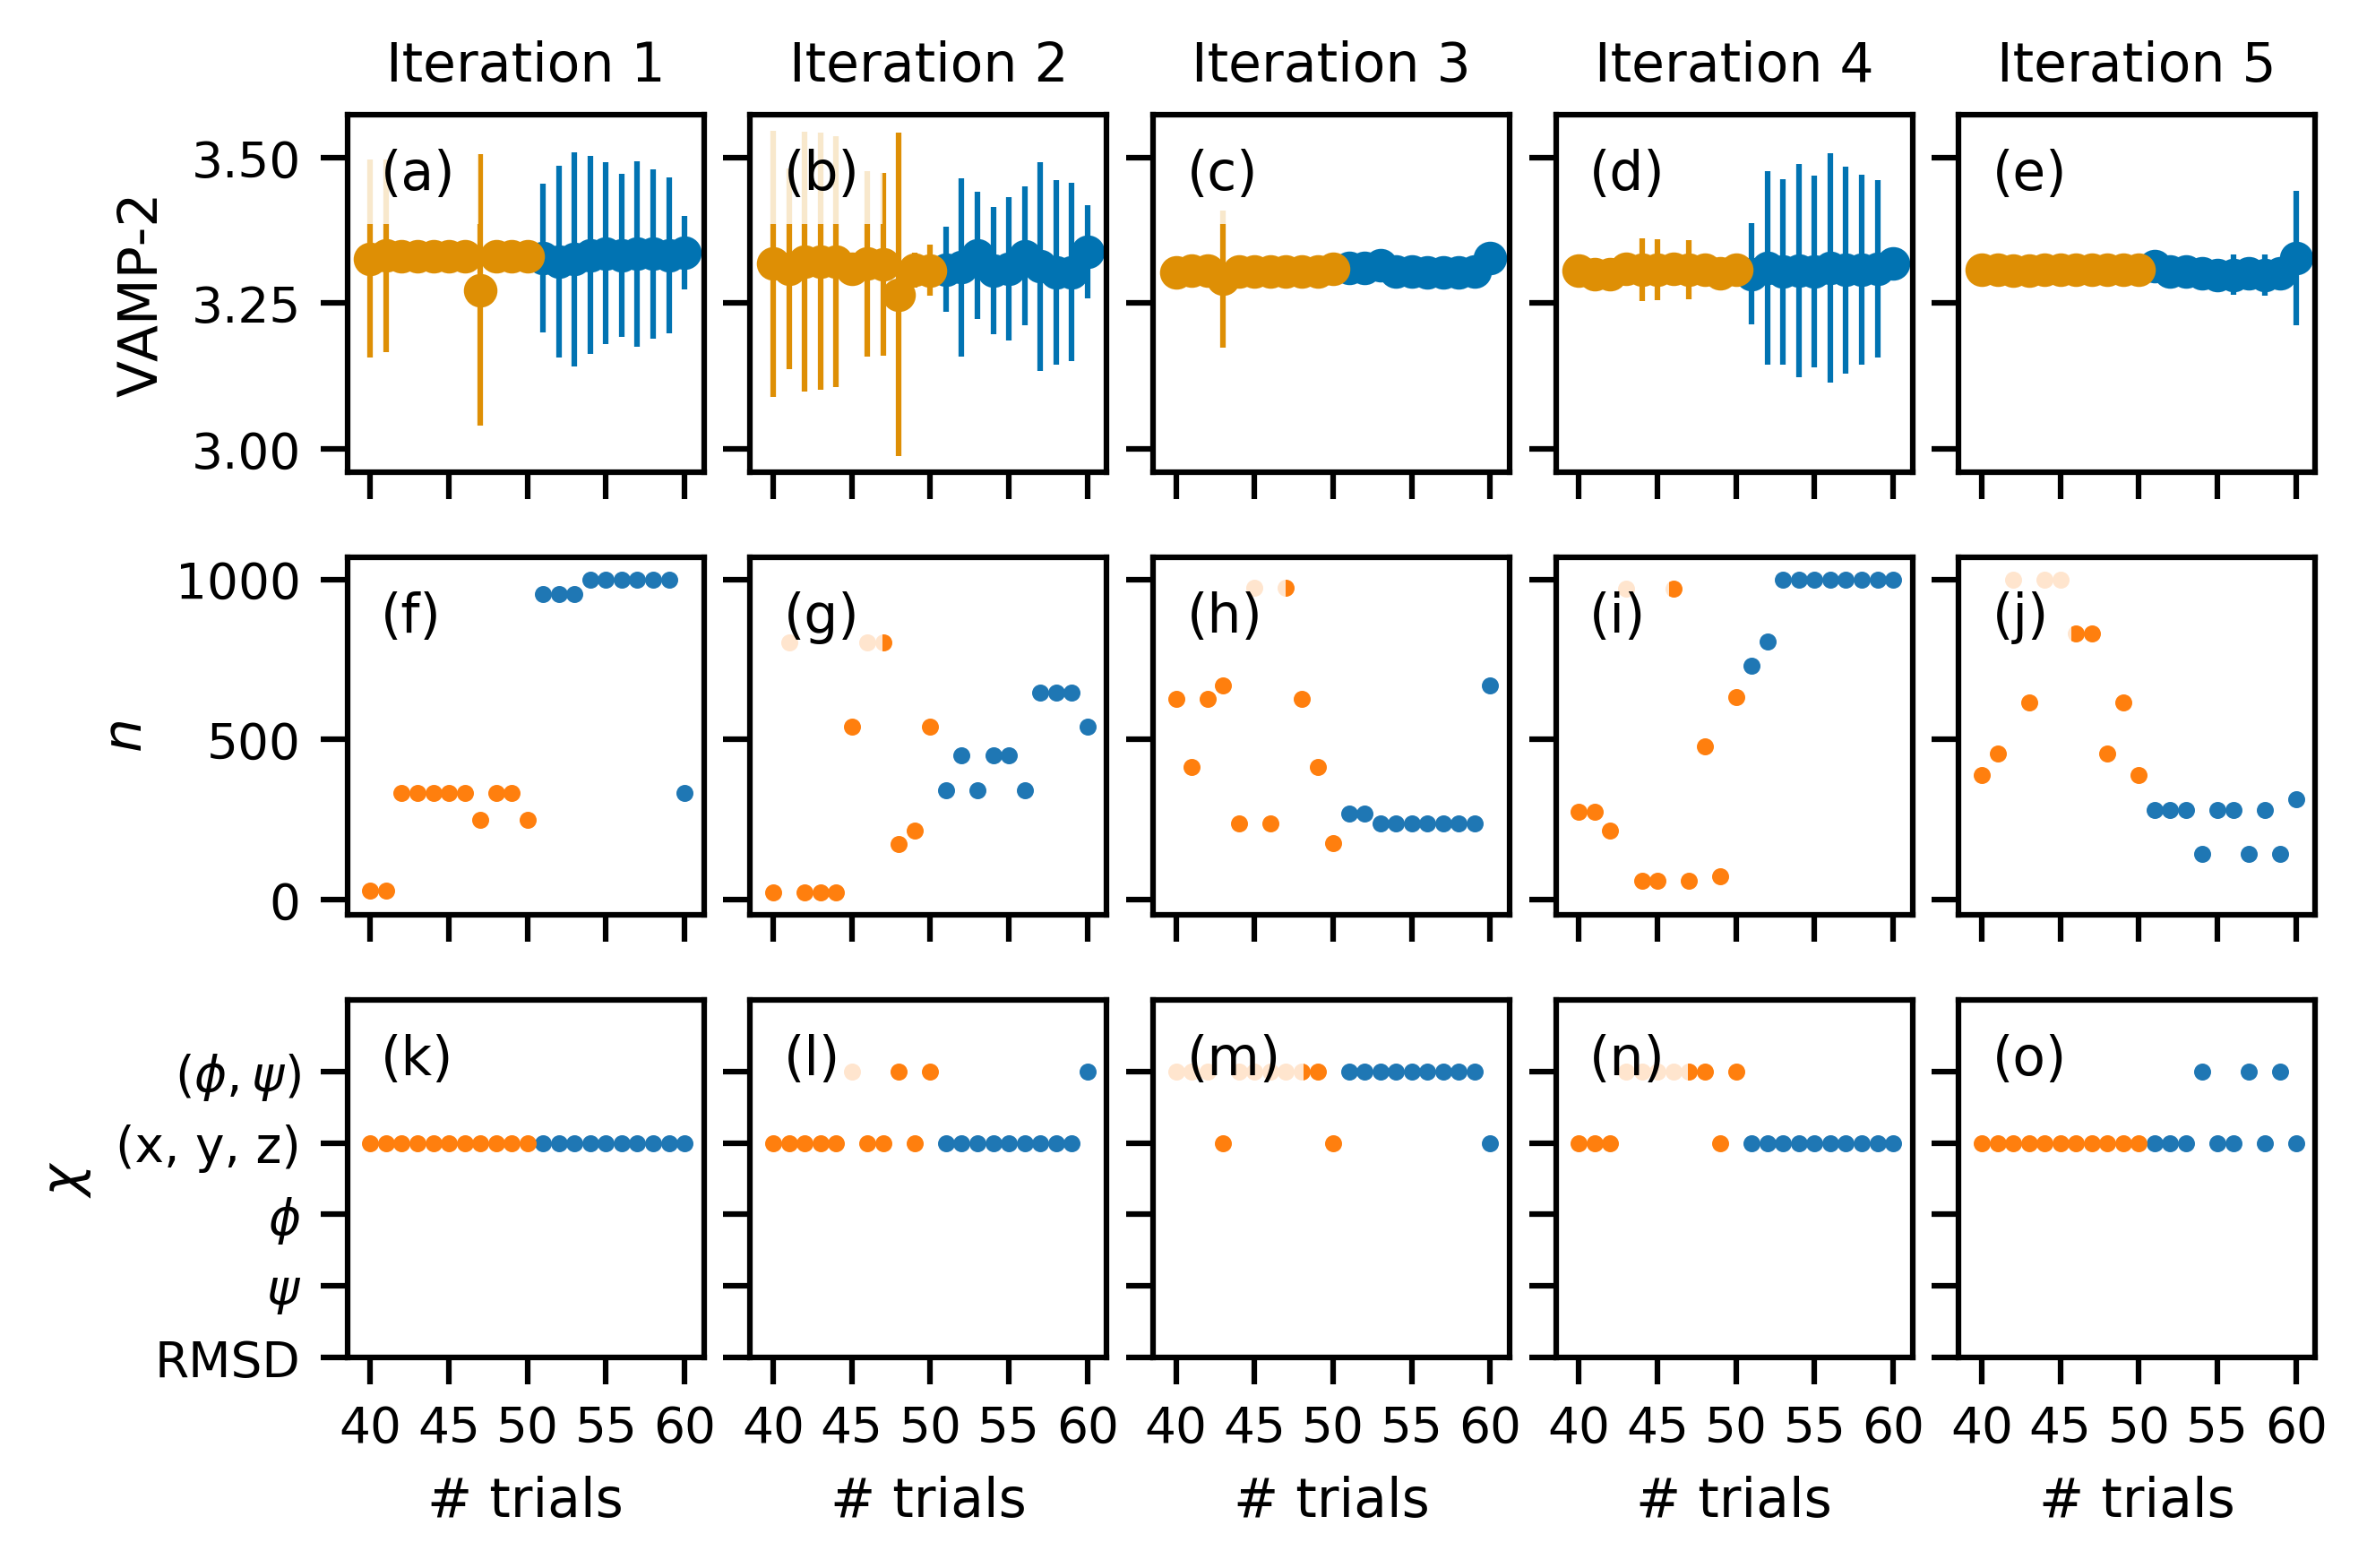
\includegraphics[width=0.7\linewidth]{chapters/msm_optimization/figures/ala1_opt_traj_start_obs_50.png}}
\end{figure}

\begin{table}
    \centering
    \caption[MSM hyperparameters for alanine dipeptide pre- and post- Bayesian optimisation]{\textsc{MSM hyperparameters for alanine dipeptide pre- and post- Bayesian optimisation}.  Each row represents a BO experiment, seeded with $N_{\mathrm{seed}}$ randomly sampled hyperparameters trials. Five iterations of optimisation were run with $N_{\mathrm{seed}}=30,\ 50$ (labelled $\# 1, 2$ etc.). The number of optimisation steps is equal to the difference in the pre/post value of $N_{\mathrm{total}}$.  The optimum of the response surface estimated with all the trial data ($N_{\mathrm{total}}=500$) is included even though it was not optimised using BO. Each column is a variable or outcome with values associated with the optimum value of $\mu$, before and after BO.  
    }
\begin{tabular}{llrrrrrrllrr}
\toprule
   &   & $N_{total}$ & & $\mu$ & & $\sigma$ & & $\chi$ &  & $n$ & \\
 $N_{seed}$  &   \#  &         Pre & Post &   Pre &  Post &      Pre &  Post &  Pre & Post & Pre & Post \\
\midrule
0  & 1 &         500 &      & 3.318 &       &    0.002 &       &     $(x, y, z)$ &              & 762 &      \\
\midrule
30 & 1 &          30 &   40 & 3.302 & 3.338 &    0.004 & 0.192 &  $(\phi, \psi)$ &     $(x, y, z)$ & 577 &  969 \\
   & 2 &          30 &   40 & 3.318 & 3.233 &    0.005 & 0.086 &  $(\phi, \psi)$ &     $(x, y, z)$ & 540 &  133 \\
   & 3 &          30 &   40 & 3.076 & 2.947 &    0.557 & 0.420 &  $(\phi, \psi)$ &  $(\phi, \psi)$ &  88 &   10 \\
   & 4 &          30 &   40 & 3.065 & 3.315 &    0.553 & 0.132 &     $(x, y, z)$ &     $(x, y, z)$ & 627 & 1000 \\
   & 5 &          30 &   40 & 3.313 & 3.258 &    0.005 & 0.194 &     $(x, y, z)$ &  $(\phi, \psi)$ & 968 &  684 \\
   \midrule
50 & 1 &          50 &   60 & 3.330 & 3.337 &    0.012 & 0.032 &     $(x, y, z)$ &     $(x, y, z)$ & 251 &  333 \\
   & 2 &          50 &   60 & 3.306 & 3.338 &    0.022 & 0.040 &  $(\phi, \psi)$ &  $(\phi, \psi)$ & 540 &  540 \\
   & 3 &          50 &   60 & 3.309 & 3.327 &    0.013 & 0.013 &     $(x, y, z)$ &     $(x, y, z)$ & 176 &  670 \\
   & 4 &          50 &   60 & 3.307 & 3.318 &    0.005 & 0.004 &  $(\phi, \psi)$ &     $(x, y, z)$ & 634 & 1000 \\
   & 5 &          50 &   60 & 3.308 & 3.327 &    0.004 & 0.058 &     $(x, y, z)$ &     $(x, y, z)$ & 390 &  314 \\
\bottomrule
\end{tabular}\label{tab:ala1_best_params}
\end{table}

Ten steps of Bayesian optimisation was performed on five, randomly sampled, subsets of the full hyperparameter trial data set with sizes $N_{\mathrm{seed}}=30\ \&\ 50$. The input warping  and kernel function used in the response surfaces for all of the Bayesian optimisation experiments were the same as those used on the full trial data set, discussed in the previous two sections.  In principle these modelling choices should be determined independently for each data set but given the simplicity of the response surface it was deemed unnecessary. 

The optimisation process can be visualised by plotting the \emph{optimisation trajectories}. Figure \ref{fig:ala_opt_traj_30} shows the optimisation trajectories after seeding with $N_{\mathrm{seed}}=30$ trials and figure \ref{fig:ala_opt_traj_50} after seeding with $N_{\mathrm{seed}}=30$ trials. The $10$ steps of Bayesian optimisation are shown in blue (horizontal axis values: $N_{\mathrm{seed}} \rightarrow N_{\mathrm{seed}}+10$) and for comparison the figure also shows, in orange, the trajectory calculated using randomly sampled trials  (horizontal axis values: $N_{\mathrm{seed}}-10 \rightarrow N_{\mathrm{seed}}$). Sub-panels (i) -  (v) show how the value of the incumbent varies with the number trials in the trail data set, the orange values contain only randomly selected hyperparameters, the blue values contains a mix of BO selected and randomly selected trials. Panels (vi) - (x) show the values of $n$ and panels (xi) - (xv) show the values of the $\chi$ associated with the incumbent. 

With $N_{\mathrm{seed}}=30$ the incumbent trajectories of iterations 2, 3, \& 5 decreased after starting BO. For all iterations seeded with $N_{\mathrm{seed}}=50$ trials the incumbent trajectories remained constant or increased. In both cases the optimal values of $\chi$ oscillated between $(\phi, \psi)$ and $(x, y, z)$, while the optimal value of $n$ did not converge to a single value across separate iterations. A value of  $N_{seed} = 50$ or $25$ observations per predictor were therefore deemed tentatively appropriate. 

There are a number of observations of the optimisation trajectories which reflect on the alanine dipeptide response surface described in section \ref{sec:ala_rsm} and the usefulness of Bayesian optimisation for this system. First, the incumbent trajectories clearly show that Bayesian optimisation does not increase the value of the incumbent by a significant amount. This is a reflection of the simple nature of the response surface and the irrelevance of the number of cluster centres. Second, the response surface (in the search space domain tested) is bimodal with peaks at $\chi=(\phi, \psi)$ torsions and $(x, y, z)$ coordinates. This is reflected in the clear lack of substantive difference between the final values of $\mu$ listed in table \ref{tab:ala1_best_params} for these two values of $\chi$.  Third, the almost complete irrelevance of $n$ as a hyperparameter is clearly shown in figure \ref{fig:ala_opt_traj_50} sub-panels (vi) to (x) in which the final values of $n$, $n \simeq 1000,\ 500\ \&\ 100$ show no clear difference in the value of the incumbent. Fourth, it is possible that with more optimisation steps it could be possible to arrive at the maximum of the response surface with less seed trial observations. While this is a possibility, the fact that Bayesian optimisation is an inherently serial algorithm, while random sampling is embarrassingly parallel, it was considered more wall-time efficient (if not CPU-time efficient) to err on the side of more random seed trial data and less optimisation steps. 

\section{Conclusions}\label{sec:msm_conc}

This chapter introduced the use of response surfaces and Bayesian optimisation for understanding and optimizing the hyperparameters of MSMs. A GP model proved a satisfactory statistical model for estimating the response surface of alanine dipeptide with two predictors $\chi$ and $n$. Using the MSLL and SMSE metrics, a Mat\'{e}rn 5-2 kernel and logarithmic warping of the hyperparameter $n$ produced the best fit to the data.  The logarithmic warping was necessary to make the stationary assumption of the GP more plausible. While GPs are usually used with continuous predictors the use of dummy coding  was demonstrated to be effective in incorporating the peptide feature, $\chi$, as a categorical predictor. The relevance, the inverse of the characteristic length-scale,  was shown to reflect the importance of each  MSM hyperparameter in determining the MSM response. For the non-categorical hyperparameter, $n$, the low relevance was a reflection of the near flat response of the MSM to changes in $n$. For the categorical predictor, the protein feature $\chi$, the low relevances of each feature was a reflection of how similar the response surfaces were \emph{conditional} on the value of $\chi$.  Two BO experiments, each consisting of five iterations of the BO procedure were performed. It was found that seeding the BO procedure with 15 hyperparameter trials led to the BO procedure deteriorating rather than optimising the hyperparameter surface. Seeding the BO procedure with 25 trial observations prevented the deterioration in the incumbent however it did not optimise the incumbent either. The hyperparameters selected by BO over each iteration were not consistent. 

The main limitation of this work is that the response surface of alanine dipeptide with the MD data used was too simple to show variation with respect to $n$.  The possible reasons for the flat response with respect to $n$ is the large volume and low temporal resolution of the trajectories. In addition, the type of clustering algorithm is known to have a large effect on the quality of an MSM \cite{husicWardClusteringImproves2017a} and the effect of this has not been investigated in this work. As a result, BO was only shown to be \emph{as good} as randomly selecting hyperparameters and fitting a response surface but not better. In addition, the model selection criteria for selecting the kernel and input warpings was simple and easily implemented but ultimately ad-hoc. A plan to address these limitations in future work is laid out in the conclusions, chapter \ref{chap:conclusions}. However, as the majority of these limitations were system dependent, they do not prevent these methods being used on AADH in chapter \ref{chap:aadh}. 

% The response surface for AADH, with four predictors ($\chi$, $\tau$, $m$ and $n$) was also fit with a GP. The conditional structure of the predictor space meant that the RMSD feature was not able to be incorporated into the response surface. This is a problem for GPs in this setting. In future work more flexible models, such as Random Forests or Tree Pazen Estimators could be used to model this conditional structure more effectively. Model selection was used to select the most appropriate GP kernel and input warping. The final selected model fit the model with varying success. Overall the model fit the data well, but for the best performing feature, $(\phi, \psi, \chi)$ dihedrals, the fit was less satisfactory. 

% The relevance of the hyperparameters revealed once again that $n$ was not important in determining the response, while the TICA hyperparameters were the most relevant. While the $(\phi, \psi, \chi)$ dihedrals and interatomic distances features were the best performing, each of the features did not have high relevance. This indicated that the response surfaces conditional on the features were similar.  The relative relevance of the hyperparameters was shown to be useful in visualising the high dimensional surface.

% Bayesian optimisation was used to in an attempt to optimise the AADH response surface. After fitting the response surface with $361$ randomly sampled hyperparameters, further Bayesian optimisation did not increase the value of the maximum of the response surface or change significantly the optimal hyperparameters. Bayesian optimisation was also used on subsets of the data and the resulting optimum hyperparameters, determined from a total of $150$ trials, were similar to those determined from the full hyperparameter trial data set. This suggests the Bayesian optimisation could be used seeded with $25$ random observations per MSM hyperparameter. Further work is needed to determine the most efficient combination of random sampling and Bayesian optimisation. 

% Once the response surface was optimised and the best performing MSM hyperparameters determined,  inspection of resulting MSM eigenvalue spectrum and the response surface suggested a number of sensitivity tests to be performed.  These tests revealed a fairly robust single dominant relaxation process with associated time-scale of $\SI{2.12}{\micro\second} (\SIrange{1.0}{5.2}{\micro\second})$. A second dominant relaxation process was not ruled out. The most relevant parameters, the TICA lag time, was also associated with changing both the qualitative and quantitative nature of the MSM. This could be an example of the Rashomon effect, something described in the MSM literature. 


% The response of an MSM to a randomly selected set of hyper-paraImeters was measured using standard the MSM metric, VAMP-2. These data were used with Gaussian process regression (GPR) to model the response surface of the MSM. Input warping and the type of kernel used in the  GPR were chosen using cross-validation of the standardised log loss and squared error metrics.  Bayesian optimisation was used to find the optimum of the response surface using the expected improvement as a hyperparameter selection policy. Once the optimum had been found and the corresponding MSM was estimated, the response surface and eigenvalue spectrum was used to explore the robustness of the optimum hyperparameters with a series of sensitivity tests. 


% \begin{table}
%     \centering
%     \caption{Summary description of the molecular dynamics data of alanine dipeptide and AADH.}
%     \begin{tabular}{|l|c|c|}
%         \hline
%          & Ala\textsubscript{1} & AADH \\
%          \hline\hline
%          No. MD trajectories & $750$ & $100$ \\
%          Total sampling time & \SI{750}{\nano\second} & \SI{10}{\micro\second} \\
%          Trajectory resolution & \SI{1}{\pico\second} & \SI{100}{\pico\second} \\
%          Temperature & \SI{300}{\kelvin} & \SI{310}{\kelvin} \\
%          Integrator & Langevin & Langevin \\
%          Ensemble & NVT & NVT \\
%          Forcefield & AMBER ff-99SB-ILDN & CHARMM-36 \\
%          Solvation & Explicit, TIP3P & Explicit, TIP3P \\
%          \hline
%     \end{tabular}
%     \label{tab:md_specs}
% \end{table}

% However, not all trials were successful (for example, if the number of TICA dimensions required, $m$, exceeded the number of dimensions of the feature, $\chi$) and these trials were ignored in the following analysis. This resulted in a final trial data set of size $N=500$ for alanine dipeptide and $N=461$ for AADH. The hyperparameter trial data sets will be denoted $\mathcal{D}_{N}(s)$ where $N$ labels the number of trials and $s$ is the name of the system. e.g., the full alanine dipeptide the hyperparameter trial data set is labelled as $\mathcal{D}_{500}(\mathrm{Ala}_{1})$. 

% meaning the response lies in the range \footnote{Recall that first eigenvalue, $\lambda_{1}=1$ and the remaining eigenvalues  $\lambda_{2,3,...} < 1$ thus $\operatorname{VAMP-2}(k=4)$ will be at least $1^2 + 0^2 + 0^2 + 0^2=1$ and at most $1^2 + 1^2 + 1^2 + 1^2=4$} $[1, k]$. For alanine dipeptide values $\tau_{\mathrm{M}}=\SI{9}{\pico\second}$ and $k=5$ were used in line with \cite{bowmanQuantitativeComparisonAlternative2013}.  For AADH values of $\tau=\SI{2}{\nano\second}$ and $k=4$ were used based on the eigenvalue spectrum of a reference MSM described in chapter \ref{chap:aadh}. 

% \begin{table}
%     \caption{The hyperparameter search space for AADH. TICA was applied to every feature except RMSD. Torsional angles, $\theta$, were given $(\sin(\theta),\cos(\theta)$ representations. The Cartesian coordinates were first aligned to a single, randomly chosen, trajectory frame so that feature (5) did not include spurious rotational or translational motion. The number of dimensions, `Dim.', refers to the number of individual feature variables created by $\chi$.}
%     \centering
%     \begin{tabularx}{0.9\textwidth}{ |>{\raggedright\arraybackslash}l|l|>{\raggedright\arraybackslash}X|c| >{\raggedright\arraybackslash}X | } 
%     \hline
%     \textbf{Hyper-parameter} & \textbf{Type} & \textbf{Range} & \textbf{Dim.} &\textbf{Details} \\
%      \hline\hline
%     Feature, $\chi$ & Categorical & (1) $(\phi, \psi, \chi)$ & $\num{116}$  & \\
%     & & (2) $|\mathbf{r}_{1}-\mathbf{r}_{2}|$  & $\num{ 2346}$& Heavy atoms inter-atomic distances \\
%     & & (3) $C_{\alpha}-C_{\alpha}$ & $\num{15}$ & alpha-Carbon contacts\\ 
%     & & (4) $X-X$  & $\num{15}$ & Heavy atoms contacts\\ 
%     & & (5) RMSD & $\num{1}$ &  Heavy atoms only\\ 
%     \hline
%     TICA lag time, $\tau$ & Integer &\SIlist[list-final-separator = { ... }]{1;1.1;100}{ns} &  & \\
%     \hline
%     TICA components, $m$& Integer &\numlist[list-final-separator = { ... }]{1;2;20} & & \\
%     \hline
%     Cluster centres, $n$ & Integer & \numlist[list-final-separator = { ... }]{10;11;1000}& &  Clustered using k-means clustering  \\
    
%      \hline
%     \end{tabularx}
%     \label{tab:aadh_searchspace}
% \end{table}


% \begin{table}
%     \centering
%     \caption{MSM model, scoring and cross validation (CV) details used in creating the hyperparameter trial data sets for alanine dipeptide and AADH. The number of trials reported is the number after removing models that failed to fit for any reason.}
%     \begin{tabular}{|c|c|c|}
%     \hline
%     & Ala\textsubscript{1} & AADH \\
%     \hline\hline
%     $\tau_{\mathrm{M}}$ & \SI{9}{\pico\second} & \SI{2}{\nano\second} \\         
%     $\operatorname{VAMP-2}(k)$ & $k=5$ & $k=4$ \\
%     No. trials & 500 & 461 \\
%     CV method & 50:50 Shuffle Split & 50:50 Shuffle Split \\
%     CV folds & 20 & 20 \\
%      \hline       
%     \end{tabular}
%     \label{tab:trial_specs}
% \end{table}


% Bayesian optimisation is a type of sequential model based \cite{hutterSequentialModelbasedOptimization2011} optimisation technique. These techniques entail first sampling the response of the objective function over a search space to create a trial data set. A statistical model called the \emph{surrogate function}, which serves as a proxy for the objective function, is built using the sampled responses. An utility function, known as the \emph{acquisition function}, determines the anticipated utility of a set of inputs in optimizing the objective function, based on the predictions and uncertainty in the surrogate function.  The objective function is then sampled using the set of inputs which maximize the acquisition function. This new trial is added to trial data set and process repeated. 


% \subsection{MSM Optimisation}
% Bayesian optimisation was used to determine whether the maximum of the response surface estimated using  could be reached by starting starting with smaller trial data set, i.e., whether 

% An exploratory optimisation procedure was first performed on the alanine dipeptide system to demonstrate its effectiveness and to determine how many randomly sampled seed trials are needed to initalise the BO procedure, $N_{seed}$. $p=10$ steps of the BO algorithm was performed on five random subsets of the alanine dipeptide trial data set with $N_{seed}=30, 50$ trials (stratified over the features $\chi$), corresponding to $15, 25$ trials per predictor. As discussed further in section \ref{sec:ala_opt}, $25$ trials per predictor was found to result in satisfactory improvement in the incumbent.  

% For AADH two optimisation experiments were performed:
% \begin{enumerate}
%     \item $p=50$ steps of Bayesian optimisation was performed using a response surface seeded with all of the randomly sampled hyperparameter trial data ($N_{seed}=361$);
%     \item $p=50$ steps of Bayesian optimisation was performed on five subsets  of the hyperparameter trial data with  $N_{seed}=100$, which corresponded to $25$ trials per predictor.
% \end{enumerate} 

% In both cases the combination of input warping and kernel-type  were determined by selecting the highest ranked model using the MSLL and SMSE metrics (equations \ref{eqn:msll} and \ref{eqn:smse}). The of the kernel hyperparameters were determined by maximizing the marginal log-likelihood, equation \ref{eqn:marg_llike}.



% Optimum MSM hyperparameters for AADH pre- and post-Bayesian optimisation (BO). Each column represents a Bayesian optimisation experiment, seeded with $N_{seed}$ randomly sampled hyperparameter trials. Five iterations of optimisation were run with $N_{seed}=100$ (labelled $\# 1, 2$ etc.) and a single iteration optimising the response surface using all the trial data ($N_{seed}=361$). Each row is a variable or outcome with values associated with the optimum value of $\mu$ before and after the BO.



% \section{Antonia Mey comments}
% \emph{Structure:}
% I think the main thing I would change,  is altering the structure a little bit to make it easier to follow (below a rough suggestion). 

% \begin{enumerate}
%     \item MSMs are great, but has too many modelling choices, here we introduce a method to alleviate this
%     \item We need MD data to create MSMs, here are the details on the MD systems
%     \item Here is how you build an MSM and based on this I have chosen a fixed MSM lag time (this may be done in a different chapter)
%     \item Now we are left with all of these other parameters how can we make sure this is the best choice of MSM?
%     \item Lets turn to ML and see if we can use GP and BO to figure out the best parameter combination
%     \item Look I came up with this amazing algorithm to do this
%     \item Let’s apply this to a) di-ala b) AADH.
% \end{enumerate}

% Maybe  a pictorial image of what your optimisation actually does, and how you assess it, much in the same way as you describe the steps of markov modelling would be useful (I am far too big a fan of diagrams and it would be a great TOC graphic for the paper). For example to be put into the introduction to the chapter.

% \emph{Core concepts}
% If you can make sure core concepts are well explained and highlighted in the text. With this I mean things such as:
% \begin{itemize}
%     \item Response surface (I didn’t quite understand)
%     \item How you make kernel choices
%     \item how you select l
%     \item Trial data 50:50 shuffle split etc. (essentially at the moment I don’t feel like I could reproduce exactly what you did to the data and how to run the optimisation. for the MSM part it seems a bit clearer, but that may just be because I have done these steps many times)
% \end{itemize}

% \emph{Nomenclature/Maths typesetting}
% I think the main confusions for me were the nomenclature of variables. Even when you redefine the nomenclature, there are many differe phi, psi and ks and xs and other. I am a fan of specific examples from time to time in the text after something is definite of what the variables are in terms of your MD data for example, or what exact optimisation variable you are referring to, even if repetitive makes it easier for the reader (and this is still a Chemistry PhD I suppose). This may be a ‘spelling thing’, but there is a lot of vectors/matrices that should be bold missing. 

% % Conclusions: where you state "something described in the MSM literature”, cite some relevant references. 

% It will be important to discuss the relevance of your findings for future MSM investigations - summarise the implications and make some clear recommendations for how others should approach simulations and MSM construction in future. Also: do your findings reveal anything about other MSM studies in the recent literature? Important to set the work in context. This may come in Chapter 6?

  
